\section{Method}
\label{sec:method}
This chapter gives the details of the network, clustering algorithms and the evaluation metrics that are utilized and examined in this thesis. 
\subsection{Network}
\subsubsection{Selection of network}
The unsupervised feature representation learning approach proposed by Guofeng Mei \textit{et. al.}\cite{mei2022unsupervised} is adapted to be used in the existing scenario at \ac{IPA}. The primary motivation behind using an unsupervised learning  methodology is that annotation of point clouds can be really challenging. To really focus on the point level features of a point cloud, it is required to have a high number of points in the point cloud. And labelling such high number of points in each point cloud in large real world datasets can be really expensive and severely inefficient. Unsupervised learning facilitates high quality feature representation without the need for humans in the loop. Moreover, sporadic and non-uniform distribution of the point clouds can also add further challenges in point-level annotation of the point clouds. Thus, in the absence of such annotations, it is impossible to get supervised feature representations for computer vision tasks.\cite{mei2022unsupervised} 

\vspace{5 mm}

An unsupervised learning approach "ConClu" is proposed in \cite{mei2022unsupervised} that learns both the local features as well as the global features of the point clouds. It is suitable to be used in this scenario, as it would require no point-level annotation of the dataset, which is unavailable in this case. To do so, it performed point-level clustering of the points clouds to generate semantically related regions within the point cloud and performed instance-level contrasting to make the network robust to its global appearance which would be explained in detail in the following subsections.\cite{mei2022unsupervised}. Other related works like \cite{zhu2016deep} also worked in the domain of learning object feature representations using autoencoders but depth images were used in such cases. \cite{mei2022unsupervised} on the other hand worked with point clouds which is similar to the ABC dataset used at \ac{IPA}. Furthermore, as mentioned in the Ch. \ref{sec:related_works}, discriminative models have the capability of distinguishing between different data augmentations. Amongst them \cite{rao2020global} and \cite{sanghi2020info3d} is seen to have promising results because of the use of contrastive learning techniques. But it is computationally expensive generate negative samples required in contrastive learning in unsupervised learning. On the other hand, the mechanism of learning the global features which encapsulate the high-level semantic information reduces the necessity to rely on negative samples of contrastive learning. Therefore, the network used in \cite{mei2022unsupervised} is deemed suitable for the task in hand.\cite{mei2022unsupervised}


\subsubsection{Architecture}
Analysing how humans perceive an object, they do not focus merely on the individual points but rather semantically related points that form a group and act as the fundamental block for the entire object as a whole. The global features focus on the entire shape of the object while the local features attains to the more detailed information in the different parts of the object. In this work, the 3D point cloud $\mathcal{\textbf{P}} = \{\textbf{p}_i \in \mathbb{R}^3| i= 1,2,3,....,N\}$, where $N$ is the number of points in each point cloud and $\textbf{p}_i$ is each point in the point cloud representated in 3D cartesian coordinate system. The point cloud $\mathcal{\textbf{P}}$ is fed to an encoder backbone $f_{\varphi}$ which generates a point-wise feature matrix $\mathcal{\textbf{F}} = \{ f_{p_i}\}_{i=1}^{N}$ where $f_{p_i}$ is the point-wise feature vector. The objective is to train a feature encoder $f_{\varphi}$, PointNet in this case, having parameters $\varphi$ in an unsupervised learning paradigm. The entire pipeline of the process is elaborated in Fig.\ref{fig:conclu_arch}.
\begin{figure}[h]
    \centering
    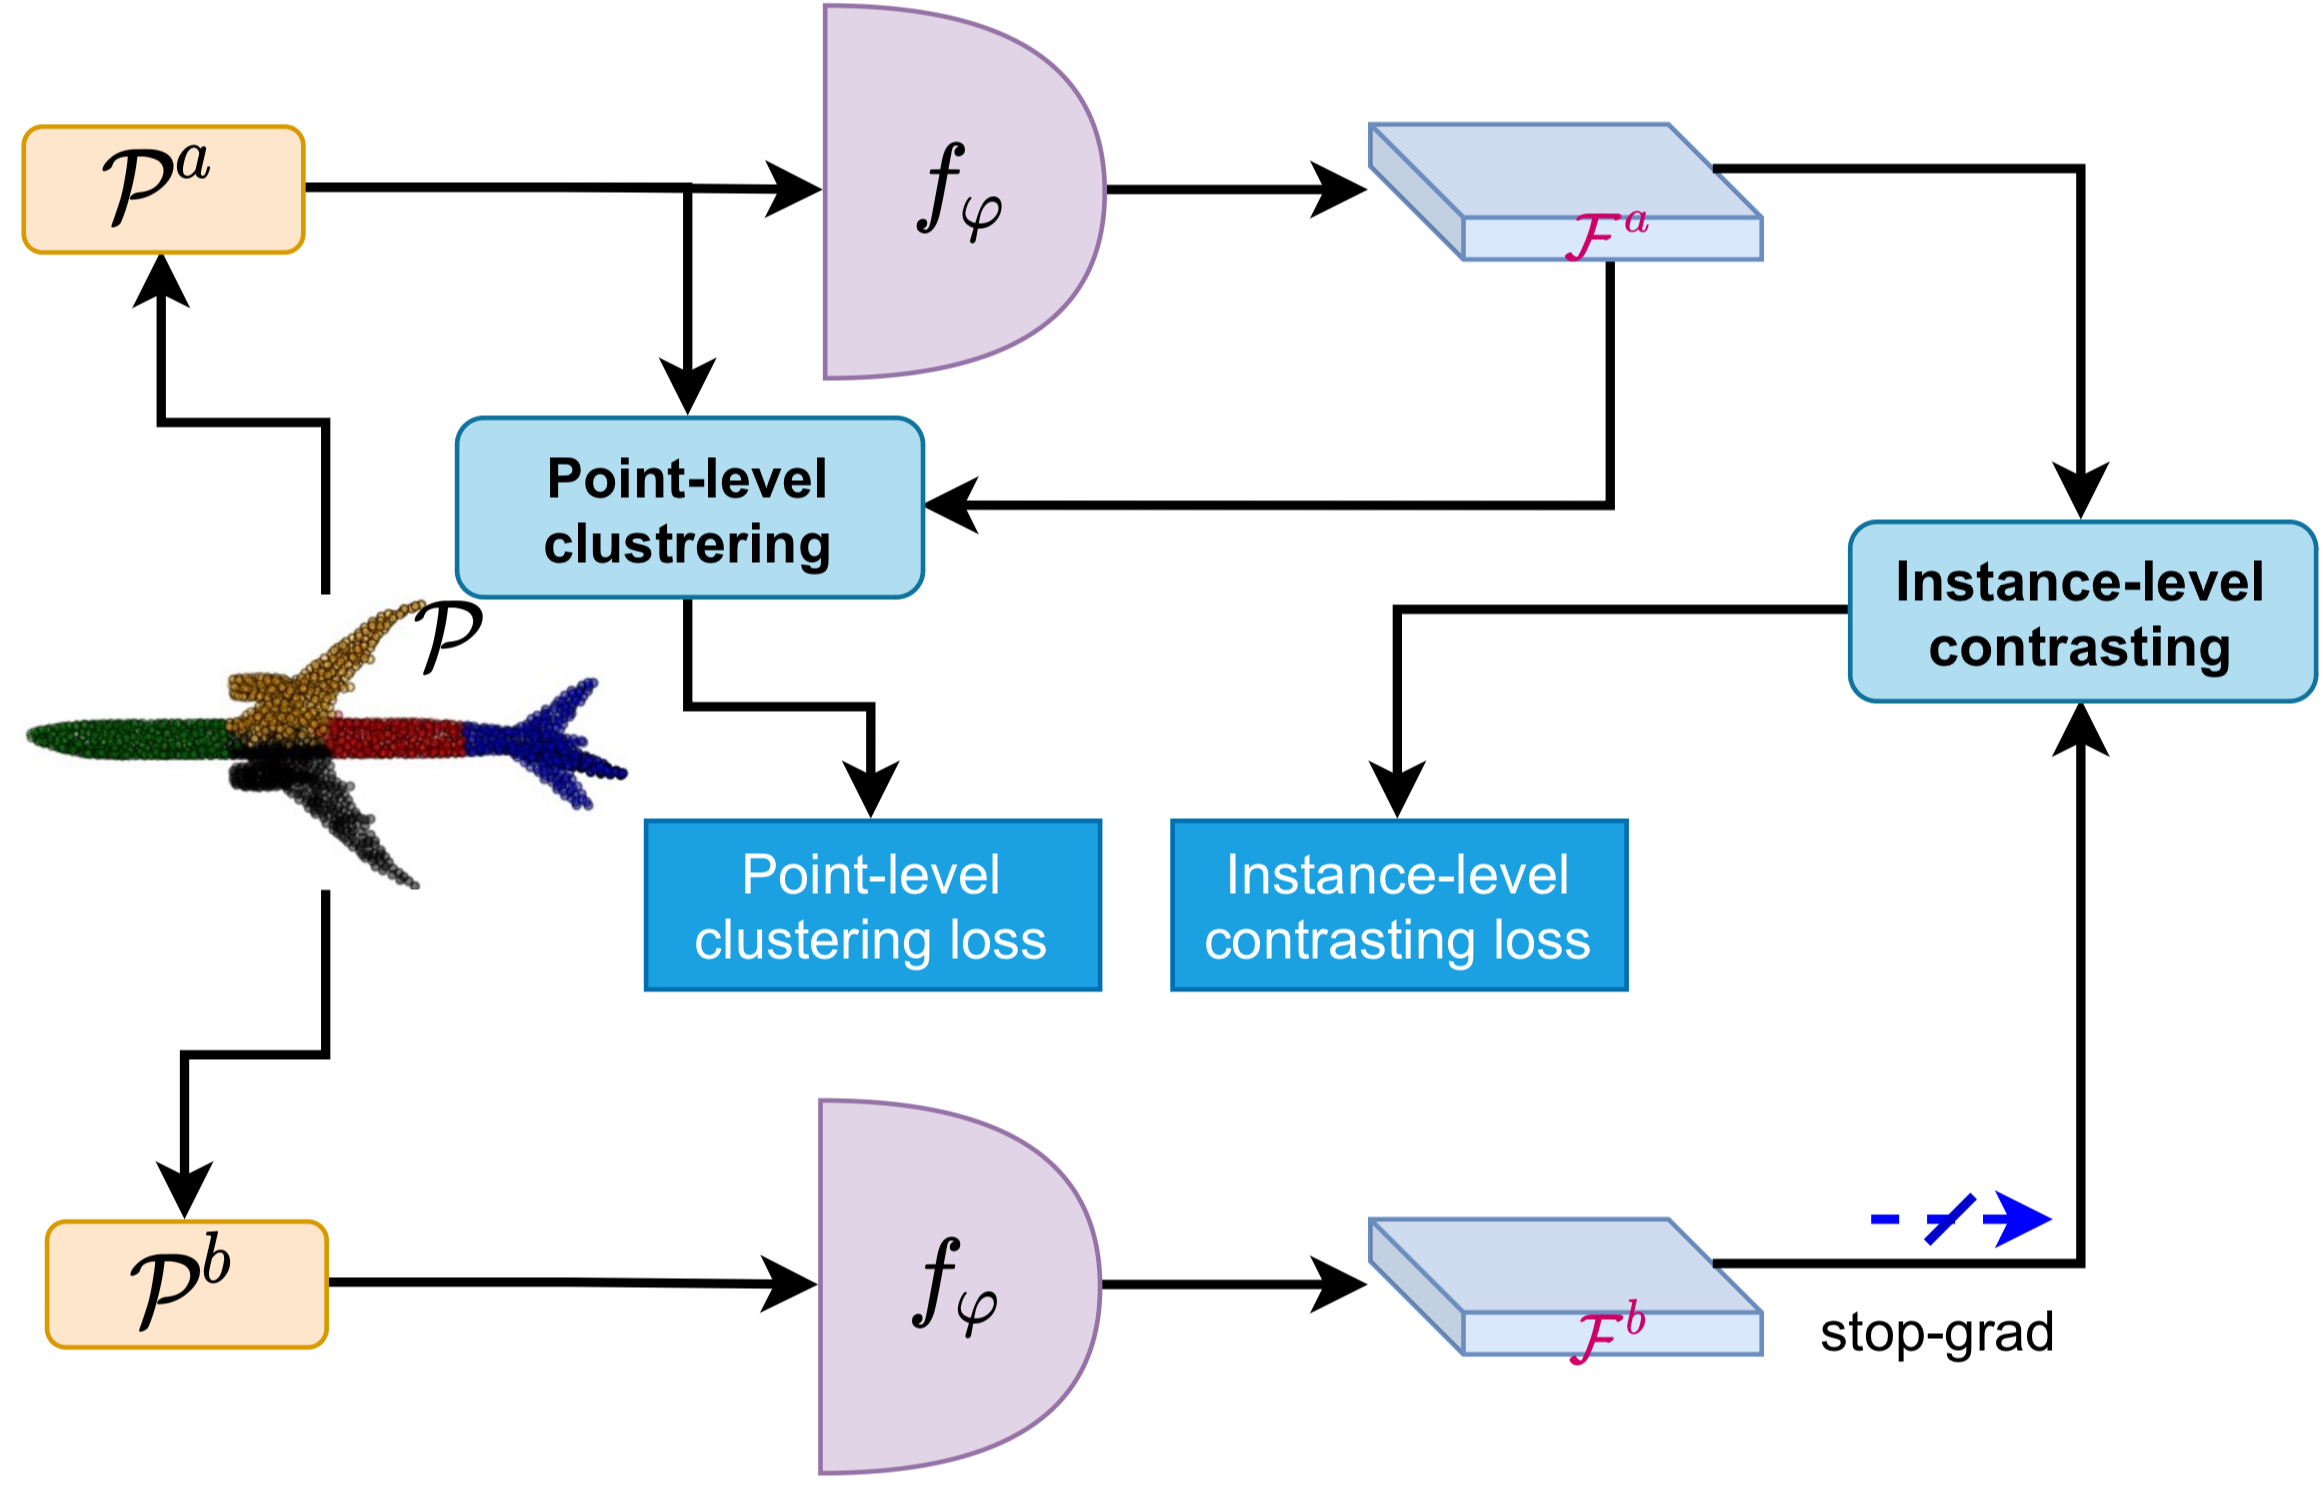
\includegraphics[width=320pt,height=200pt]{pictures/conclu_arch.jpg}
    \caption{The ConClu model pipeline including the two modules: point -level clustering and instance-level contrasting.\cite{mei2022unsupervised}}
    \label{fig:conclu_arch}
\end{figure} 
 As it can be seen that the architecture has two main parts: the point-level clustering for learning the local features and the instance-level contrasting for learning the global features. Before a detailed analysis of each module is given, here is a brief overview of the entire process. The augmented views $\mathcal{\textbf{P}}^a$ and $\mathcal{\textbf{P}}^b$ are obtained for each point cloud $\mathcal{\textbf{P}}$ and are fed to the encoder $f_{\varphi}$ such that it generates the feature matrices $\mathcal{\textbf{F}}^a$ and $\mathcal{\textbf{F}}^b$ respectively. Thus, the inputs to the point-level clustering are $\mathcal{\textbf{P}}^a$ and $\mathcal{\textbf{F}}^a$. It is to be noted here that the feature encoder $f_{\varphi}$ shares the weights between the two augmented views. $f_{\varphi}$ is trained in a way such that it minimizes the point-level clustering and the instance-level contrasting loss together. It is also to be noted here, that the encoder receives the gradient only from the top branch. After the training is completed, both the loses are cast aside and only the encoder is needed for further tasks.\cite{mei2022unsupervised}

\subsubsection{Encoder Backbone}
Keeping in line with \cite{mei2022unsupervised}, two feature representation learning backbones are used for the experiments, the PointNet \cite{qi2017pointnet} and the \ac{DGCNN} \cite{wang2019dynamic} backbone. The mechanism and the architecture of the feature extraction backbones are elaborated further in the following sections.
\subsubsection*{PointNet Autoencoder}

For the purpose of weight sharing and other kernel optimization methods, traditional convolution networks need extremely regular formats for the input data as prevalent in \ac{RGB} or depth images and 3D voxels. But point clouds are not regular data structures. It is just a set of 3D points which is permutation invariant to its constituent points. Or in other words, the order in which the individual points of a point cloud are processed is inconsequential. In \cite{qi2017pointnet} the authors suggested an end-to-end architecture that accepts the point clouds as input and generates the class label of the entire object or a class label for each of the individual points in the point cloud. The PointNet architecture is shown in Fig. \ref{fig:pointnet_arch}.
\begin{figure}[t]
    \centering
    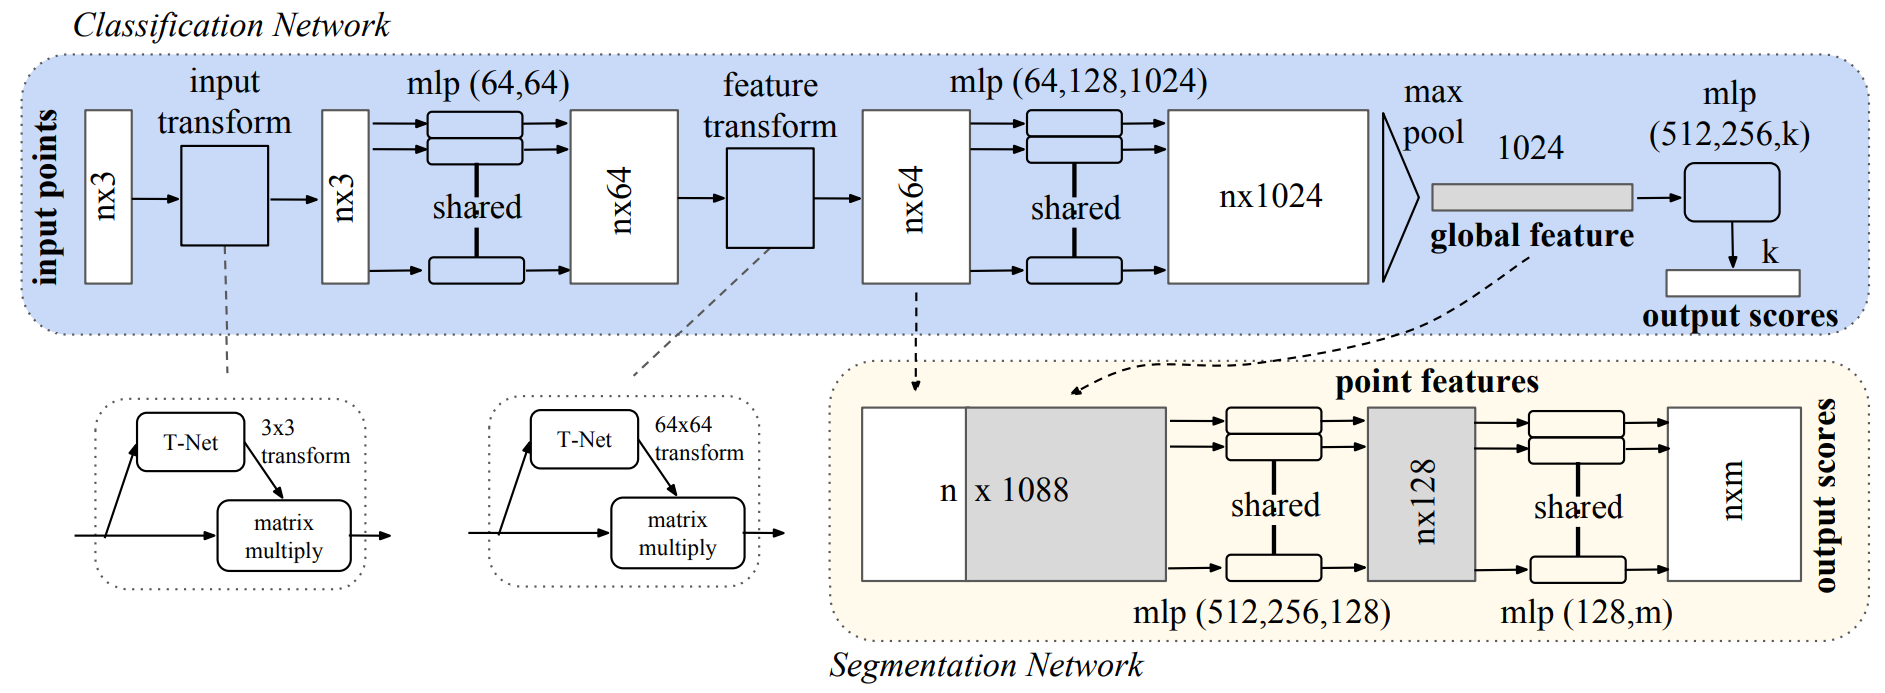
\includegraphics[width=400pt,height=250pt]{pictures/PointNet.png}
    \caption{The PointNet Architecture.\cite{qi2017pointnet}}
    \label{fig:pointnet_arch}
\end{figure}
It consists of three important modules:
\begin{itemize}
    \item a symmetric function to aggregate information, 
    \item a module that integrates the local and the global features, 
    \item an alignment network that orients the points of the point cloud and their features. 
\end{itemize}
A further detailed overview of each of the building blocks are given in the following passages.

\vspace{5mm}

\textbf{Symmetry function} The points in the point cloud are an unordered set of points, which means the order in which they appear is irrelevant. Therefore, to make the network invariant to permutation, the following approaches could be adopted. 
\begin{itemize}
    \item The input points could be sorted in canonical manner. Sorting the points isn't an efficient solution because in high dimension space there isn't actually any stable ordering w.r.t the point perturbations. Contradiction is a simple way to demonstrate that. If such an ordering existed, it would mean there is a bijection mapping between the higher dimension space and a 1d real line. For this ordering to be stable, the bijection mapping would need to maintain spatial proximity even if the dimensions decreased in the event of point perturbations. This is not feasible in most cases. As a result, sorting only partially fixes the ordering problem and it brings additional challenges for the network to learn a consistent bijection mapping between the input and the output.\cite{mei2022unsupervised}
    \item The second approach is to treat the points as a sequential data and training a \ac{RNN} with different randomly permuted input sequence in order to make it invariant to the order in which the input appears. But in \cite{vinyals2015order} it is proved that the order indeed matters and cannot be overlooked completely. Moreover, even if a \ac{RNN} is robust to the order of the input with small length(e.g. dozens), it suffers from scalibility issues. It can't be scaled to inputs with high number of elements as it is in point clouds.\cite{mei2022unsupervised}
    \item The data from each point could be combined using a symmetric function. Binary addition and multiplication are some examples of symmetric functions. Hence, the idea proposed by the authors in \cite{qi2017pointnet} is to devise a symmetric function on the transformed set of points to approximate the general function defined on the points as in Eq. \ref{eq:sym_func}.\cite{mei2022unsupervised}
\end{itemize}
   
\begin{equation}
    \label{eq:sym_func}
    f(\{x_1, ...., x_n\}) \sim g(h(x_1), ...., h(x_n)),
\end{equation}
where $\mathit{f}: 2_{\mathbb{R}_{\mathit{N}} \rightarrow \mathbb{R}}, \mathbb{R}^{\mathit{N}} \rightarrow \mathbb{R}^{\mathit{K}}$ and $g: \underbrace{\mathbb{R}^{\mathit{K}} \times ... \times \mathbb{R}^{\mathit{K}}}_\text{n} \rightarrow \mathbb{R}$ is the symmetric function. Here $h$ is a multi-layer perceptron network and $g$ is a combination of a single variable function and a max pooling function. Even if this module is fairly simple, it has some of the very important implications. If $\mathit{C_S}$ is the set of critical points, the points which contributed to the max pooled feature, the PointNet architecture is seen to be quite robust to the non-critical points. In other words, discarding the non-critical points don't lead to any loss of information about the global shape of the object as shown in Fig. \ref{fig:critical_points}. 

\begin{figure}[t]
    \centering
    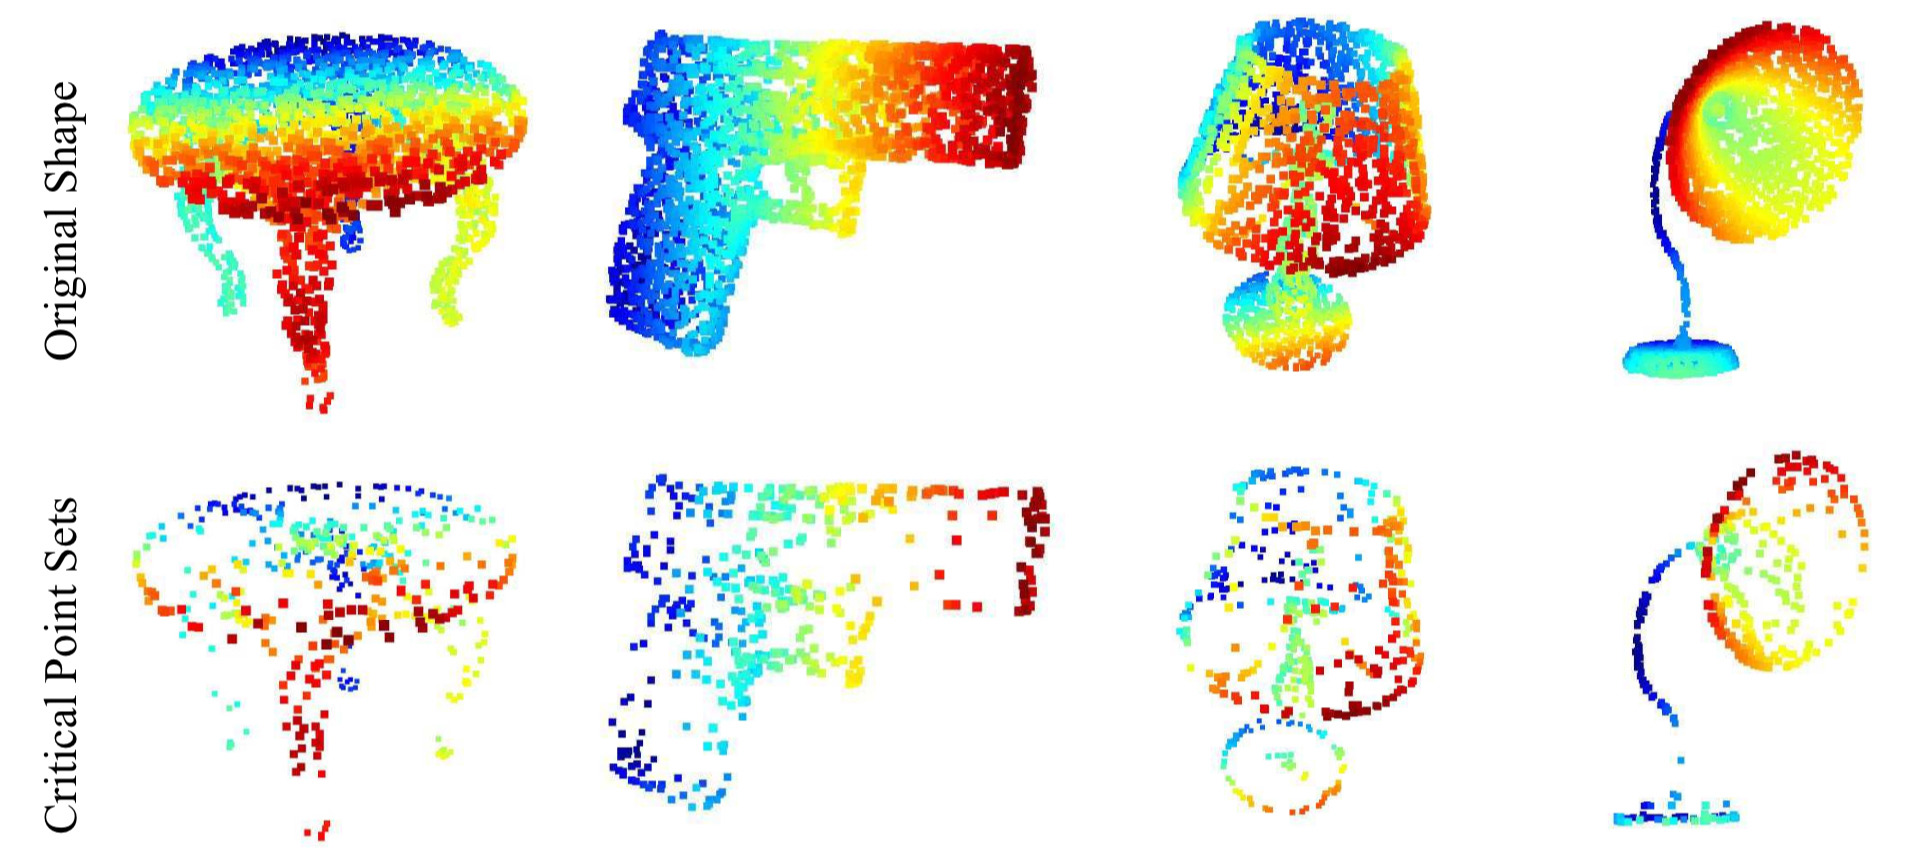
\includegraphics[width=300pt,height=150pt]{pictures/critical_points.jpg}
    \caption{Critical points set and the original shape.\cite{qi2017pointnet}}
    \label{fig:critical_points}
\end{figure}

\vspace{5mm}

\textbf{Local and Global Information Aggregation} The output of the symmetry function is a vector $[\mathit{f_1, ... , f_K}]$ which is the global feature representation of the point cloud. But to get a point-wise segmentation, information about both the local features and the global features are necessary. The local features are learnt by the network in the \textit{Segmentation Network} module as shown in Fig. \ref{fig:pointnet_arch}. Once the global feature vector of the point cloud is calculated, it is concatenated with each of the point features and is fed into the network. This enables the network to learn new point-level features when it is informed about both the local and the global information. Because of this module, the network is able to predict the class probability of individual point based on both the local geometry of the object as well as the semantic region it belongs to on a global-level.\cite{qi2017pointnet}

\vspace{5mm}

\textbf{Joint Alignment Network} The network should be invariant to certain geometric transformations like rigid body transformations. A trivial solution to this issue is aligning every input set to a canonical order prior to feature extraction. But this would require an additional layers for aligning all input sets. On the contrary, the authors in \cite{qi2017pointnet} utilized a "mini-network" (\textit{T-net}) as shown in Fig. \ref{fig:pointnet_arch}. This predicts a transformation matrix which is then applied to the coordinates of the points in the point cloud. The mini-network takes after the main network and is made up of point independent feature extraction module, max pooling layers and the fully connected layers. To align the point-features from different point cloud sets, another alignment network could be introduced. It would predict the transformation matrix required for the alignment. But that would significantly increase the difficulty of optimization since the transformation matrix has much higher dimensions as compared to the spatial transformation matrix. To circumvent this issue, a regularization term is used in the softmax training loss. The constraint enforced in this case is that the feature transformation matrix is to be approximated by an orthogonal matrix as given in Eq. \ref{eq:loss_reg}.
\begin{equation}
    \label{eq:loss_reg}
    L_{reg} = \lVert I - AA_T \rVert _F^2,
\end{equation}
where $\lVert . \rVert _F$ is the Frobenius-norm, $I$ is the Identity matrix and $A$ is the feature alignment matrix predicted by the mini-network. The feature transformation matrix has been approximated by an orthogonal matrix because orthogonal transformations ensure that no information about the input is lost.

\subsubsection*{Dynamic Graph Convolutional Neural Network}
Another more general feature encoder is used in this work. It is seen that the PointNet architecture treated each point of the point cloud independently. The model is made invariant to the different possible permutations by applying a symmetric function to aggregate the features. But a limitation to this method is that it doesn't take into consideration the topology of the points. It ignores the connectedness in between the points and thus, cannot learn the local features. This limitation is addressed by Y. Wang \textit{et al.} in \cite{wang2019dynamic}. The authors proposed the EdgeConv operation which is able to learn the local features of the point cloud while still meeting the requirement of being permutation invariant. EdgeConv generated the edge features which are capable of capturing the topological information of the points i.e. the connection between a point and its neighbors. In other words, the EdgeConv operation computes a local graph for each of the points in the point cloud which is capable of learning the edge embeddings for the edges in the graph. So the model group points based on both the Euclidean distance between the points and also how they are semantically related. The EdgeConv is a plug-and-play module that would be used combined into any existing model architecture to further enhance its performance. The approach has been further elaborated in the following passages.

\vspace{5mm}

Unlike PointNet, the \ac{DGCNN} network captures the topological information by generating a local neighborhood graph and then applying an operation analogous to the convolution operation on the edges connecting a pair of points. It is in line to the methodology used in graph neural networks. But unlike a traditional graph \ac{CNN}, the local neighborhood graph is not fixed in this case. On the contrary, it is updated after every layer in the network. This is because the k-nearest neighbors of a point doesn't remain the same after every layer of the network. This happens as the k-nearest neighbors are based on the Euclidean distance between the points but rather of the proximity of the points based on the learnt embeddings. In other words, the proximity of the points in the feature space are different from the proximity of the input points in the Euclidean space. This is responsible for the non-local flow of information through the point cloud. 

\vspace{5mm}

\textbf{Edge Convolution}  In this work, the 3D point cloud $P = {p_i \in \mathbb{R}^F|i = 1, 2, 3, ...., N}$ where $N$ is the number of points in each point cloud and $p_i$ is each point in the point cloud represented in 3D cartesian coordinate system where $p_i = (x_i,y_i,z_i)$. In this work $F=3$ but it is also possible to include additional information about the coordinates such as surface normals, color, etc. Like most traditional deep neural networks, each layer acts upon the outputs of the previous layer. So generally speaking, $F$ is the dimension of the features of a particular layer in the network. The architecture of the model used in this work is shown in Fig. \ref{fig:dgcnn_arch}. The top branch is used for the classification of the point cloud and the bottom branch is for the point-wise segmentation task. The classification task requires the $n$ points in point cloud as input. $k$ is pre-defined as the number of nearest neighbors that are to be considered for generating the edge features. The EdgeConv layer computes an edge feature set of size $k$ for each point $p_i$ in the point cloud. An aggregation operation is performed on each of these sets to get the EdgeConv response for the respective points. A global aggregation function is applied on the output of the last EdgeConv layer to generate a 1D global feature descriptor. This is used to compute the classification score for $c$ classes. The point-wise segmentation branch  further extends the classification branch by concatenating the 1D global descriptor with all EdgeConv responses (acts as local descriptors) for each point in the point cloud. Thus, it generates a point-wise classification score for $p$ semantic classes that it can belong to. $\oplus$ is the concatenation operation. The spatial transform block is the module used to align the input point cloud to a canonical space. It is done by applying an estimated $3 \times 3$ transformation matrix. The coordinates of each of the points in the point cloud are concatenated with the difference in the coordinates with the $k$ neighboring points giving rise to a tensor. This tensor is used in computing above-mentioned transformation matrix. The input point cloud of shape $n \times f$, here $(f=3)$ is fed to the EdgeConv block which computes the edge features for each of the points in the point cloud. A \ac{MLP} is used for this purpose where the number of neurons in a layer is defined as $\{a_1, a_2, ... , a_n\}.$ The output of this block is a tensor with shape $n \times a_n$ after performing a pooling operation on the neighboring edge features.  
\begin{figure}[t]
    \centering
    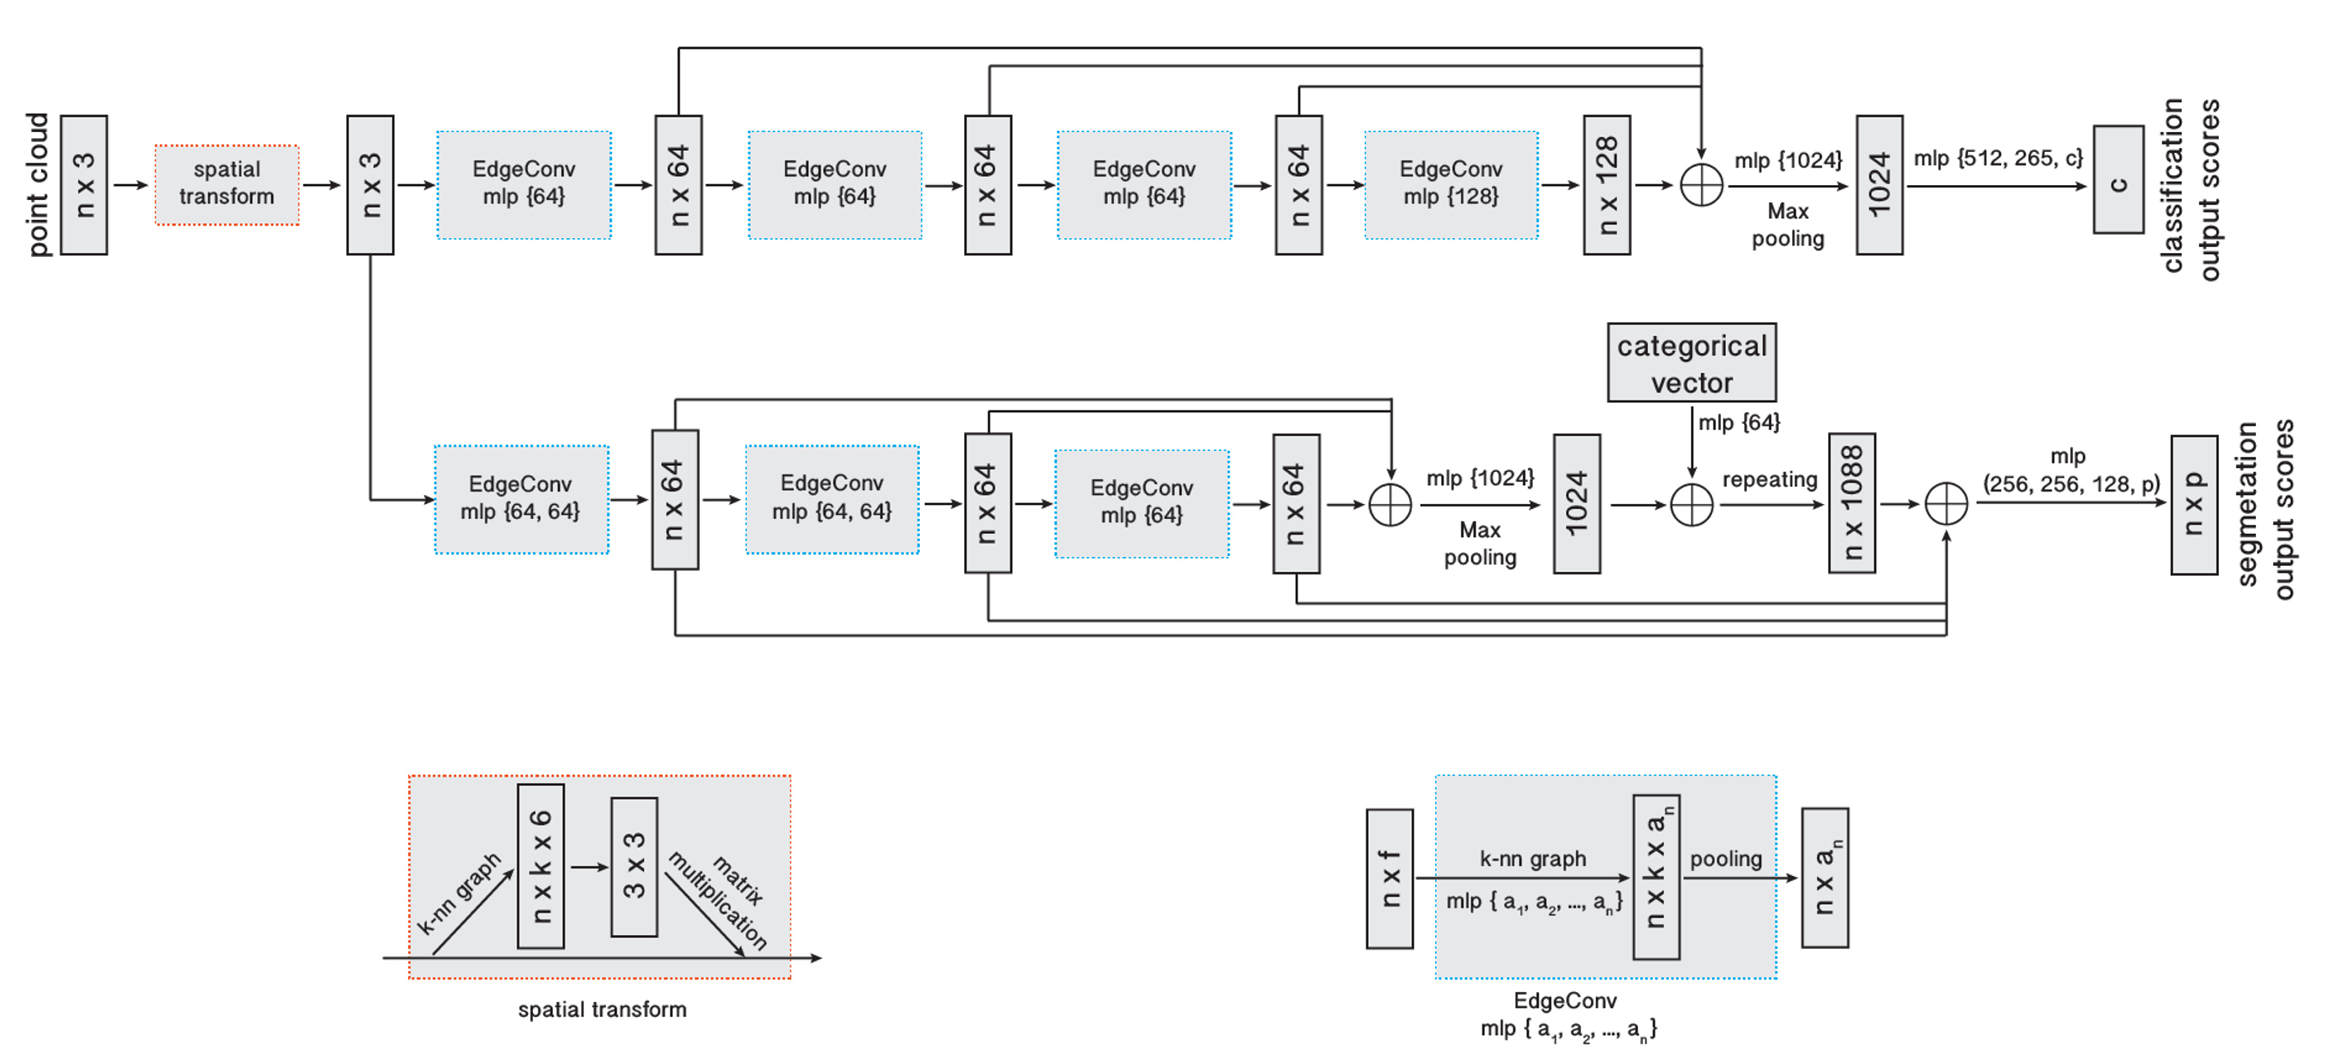
\includegraphics[width=430pt,height=300pt]{pictures/dgcnn_arch.jpg}
    \caption{The \ac{DGCNN} Architecture.\cite{wang2019dynamic}}
    \label{fig:dgcnn_arch}
\end{figure}

\vspace{5mm}

A directed graph $G = (V,E)$ which captures the topology of the point cloud where $V=\{p_i | i = \{1,2,...,n\}\}$ is the set of vertices and $E \subset V \times V$ is the set of edges. The graph $G$ is the \ac{k-NN} graph of $\mathcal{P}$ in $\mathbb{R}^F$. The graph has self-loops which means, each point in the point cloud has an edge to itself. The edge features computed by the EdgeConv block is defined as $e_{ij} = h_{\theta}(p_i, p_j)$ where $h_{\theta}: \mathbb{R}^F \times \mathbb{R}^F \rightarrow \mathbb{R}^{F'}$ is a non-linear function with a set of trainable parameters $\theta$. The EdgeConv operation is defined as a symmetric aggregation operation $\square$ which is applied on a channel wise manner. Summation or max are some of the examples of aggregation functions. It is applied on the edge features associated with all the edges that orginate from each connected vertex. Therefore, the output of the EdgeConv layer for $i$-th vertex is given by Eq. \ref{eq:EdgeConv}
\begin{equation}
    \label{eq:EdgeConv}
    p'_i = \underset{j:(i,j) \in E}{\square} h_{\theta}(p_i, p_j).
\end{equation}
Drawing similarity with convolution on images, $p_i$ is the central pixel and $\{p_j:(i,j) \in E\}$ is a patch around the central pixel as shown in Fig. \ref{fig:EdgeConv_op}. Therefore, for a point cloud with $F$ dimensions and $n$ points in it, the EdgeConv layer generates a point cloud with $F'$ dimensions and $n$ points in it.
\begin{figure}
    \centering
    \begin{minipage}[t]{.45\textwidth}
      \centering
      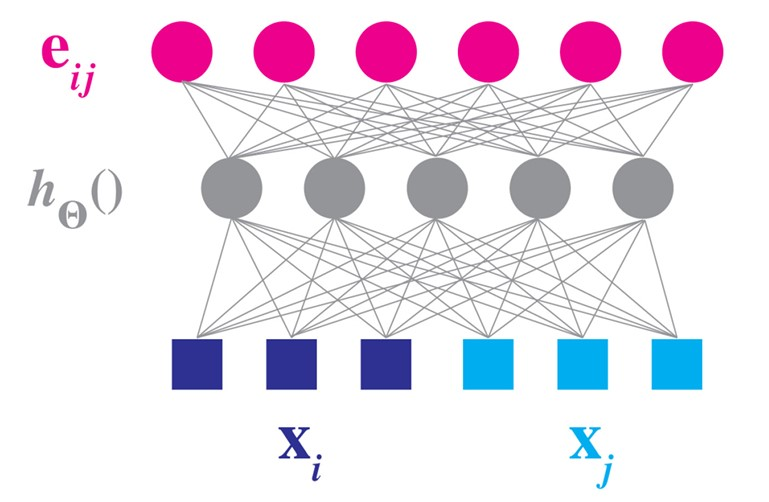
\includegraphics[width=200pt,height=120pt]{pictures/EdgeConv.jpg}
      \captionof{figure}{The Computation of edge feature $e_{ij}$ from a pair of points $p_i$ and $p_j$. Here, $h_{\theta}$ is a fully connected layer and the weights associated with it are the trainable parameters $\theta$.\cite{wang2019dynamic}}
      \label{fig:EdgeConv}
    \end{minipage}%
    \hspace{5mm}
    \begin{minipage}[t]{.45\textwidth}
      \centering
      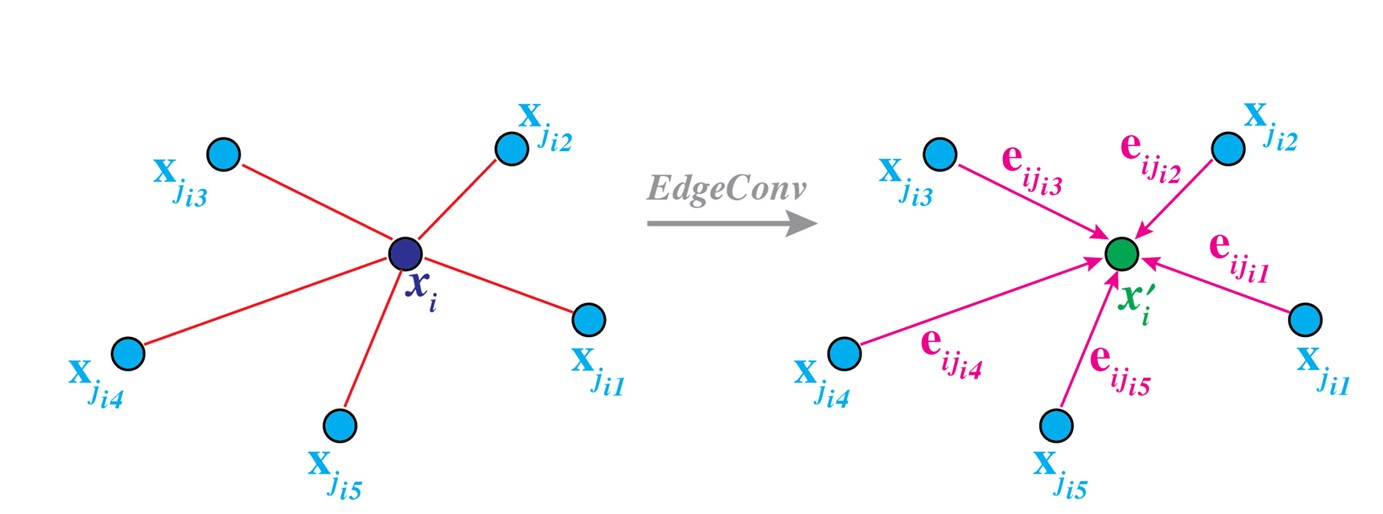
\includegraphics[width=200pt,height=150pt]{pictures/EdgeConv_op.jpg}
      \captionof{figure}{The EdgeConv operation. The output of EdgeConv is computed by aggregating the features associated with all the edges that orginate from each connected vertex.\cite{wang2019dynamic}}
      \label{fig:EdgeConv_op}
    \end{minipage}  
\end{figure}

\vspace{5mm}

Deciding the non-linear function $h_{\theta}$ and the symmetric aggregation function $\square$ plays a pivotal role in deciding the properties of the EdgeConv layer. To further illustrate on this point, if $p_1, ..., p_n$ are the points in the point cloud and the graph $G$ encapsulates the topological information of patches of fixed size around each central pixel, then if $\theta _m \cdot p_j$ is chosen as the non-linear function and sum is chosen as the aggregation operation, then it would behave as a standard convolution operation as in Eq. \ref{eq:std_conv}.
\begin{equation}
    \label{eq:std_conv}
    p'_{im} = \sum_{j:(i,j) \in E}\theta _m \cdot p_j,
\end{equation}
where $\theta = (\theta _1, \theta _2, ... , \theta _M)$ are the weights of $M$ different filters used in the convolution operation. Each entry in $\theta _m$ has the dimensionality as $p_i$ and $\cdot$ is the Euclidean inner product. Another variation of $h$ could be Eq. \ref{eq:EdgeConv_pointnet}. 
\begin{equation}
    \label{eq:EdgeConv_pointnet}
    h_{\theta}(p_i, p_j) = h_{\theta}(p_i).
\end{equation}
Here only the global embedding is taken into consideration and the non-linear function is unaware of the local features. This happens in PointNet and thus, it could be considered as a special case of EdgeConv. Another variation of $h$ as adapted by Atzmon \textit{et al.} in \cite{atzmon2018point} is Eq. \ref{eq:EdgeConv_gaussian} and Eq. \ref{eq:EdgeConv_gaussian_point}.
\begin{equation}
    \label{eq:EdgeConv_gaussian}
    h_{\theta}(p_i, p_j) = h_{\theta}(p_j).
\end{equation}
and 
\begin{equation}
    \label{eq:EdgeConv_gaussian_point}
    p'_{im} = \sum_{j \in V}(h_{\theta (p_j)})g(u(p_i,p_j)).
\end{equation}
Here $g$ is a Gaussian distribution kernel and $u$ calculates the pairwise Euclidean distance between the points in the point cloud. Another variation of $h$ could be to only capture the local features and ignore the global features based on the fact that the global shape is a collection of the local patches as shown in the following Eq. \ref{eq:EdgeConv_local}.
\begin{equation}
    \label{eq:EdgeConv_local}
    h_{\theta}(p_i, p_j) = h_{\theta}(p_j-p_i).
\end{equation}
The final variation of $h$ which is utilized by the authors in \cite{wang2019dynamic} is an asymmetric edge function as shown in Eq. \ref{eq:EdgeConv_asym}.
\begin{equation}
    \label{eq:EdgeConv_asym}
    h_{\theta}(p_i, p_j) = \bar{h_{\theta}}(p_i, p_j-p_i).
\end{equation}
This explicitly takes into account the global feature information as in Eq.\ref{eq:EdgeConv_pointnet} captured by the coordinates of the central pixel of the patch $p_i$ and the information of the local neighborhood as in Eq. \ref{eq:EdgeConv_local} and is captured by $p_j-p_i$. The EdgeConv operator is defined as 
\begin{equation}
    \label{eq:EdgeConv_op}
    e'_{ijm} = \ac{ReLU}(\theta _m \cdot (p_j - p_i) + \phi _m \cdot p_i).
\end{equation}
This operator could be implemented as a shared \ac{MLP} and then performing a max-pooling operation as in Eq. \ref{eq:EdgeConv_max}.
\begin{equation}
    \label{eq:EdgeConv_max}
    p'_{im} = \underset{j:(i,j) \in E}{max}e'_{ijm},
\end{equation}
where $\theta = (\theta _1, \theta _2, ... , \theta _M)$ are the weights of $M$ different filters used in the convolution operation.

\vspace{5mm}

\textbf{Dynamic Graph Update} A crucial point in this network is to regenerate the graph using \ac{k-NN} in the feature space after each layer. This is the main difference of this network as compared to traditional graph \ac{CNN} for which there is a fixed graph for all the layers of the network. Because the graph is updated after every layer, the architecture gets its name the \ac{DGCNN}. With dynamically updating the graph after each layer, the receptive field increases to as large as diameter of the point cloud, even if the points in the point cloud are sparse. Thus, after each layer a different graph is computed $G^{(l)} = (V^{(l)}, E^{(l)})$, where $G^{(l)}$ is a graph in the $l$-th layer with vertices $V^{(l)}$ and edges $E^{(l)}$ which can be denoted as $(i,j_{i1}), ... , (i,j_{ik_{l}})$ such that $p_{j_{i1}}^{(l)}, ... , p_{j_{ik_{l}}}^{(l)}$ are the k-nearest points closest to point $p_i$ at layer $l$. In other words, the model constructs a different graph for each point in the point cloud after every layer where the nearest points and the edges emerging from a vertex(point in the point cloud in the case) changes at every layer. A pairwise distance matrix in the feature space is used to calculate the k-nearest points of each point in the point cloud. As a result of this, the network has the following properties,
\begin{itemize}
    \item \textit{Invariant to permutations}. The output of an EdgeConv layer is given by
    \begin{equation}
        \label{eq:EdgeConv_perm}
        p'_{i} = \underset{j:(i,j) \in E}{max}h_{\theta}(p_i,p_j). 
    \end{equation}
    Because of the usage of a max operator which is symmetric in nature, the output of the layer $p'_{i}$ is permutation invariant to the order in which $p_i$ appears in the input point cloud. Other functions which are symmetric (eg. $\sum$) in nature can also be applied here instead of max. The global max pooling operator used to aggregate point features is a symmetric function and thus, gives permutation invariant results.
    \item \textit{Invariant to translation.} The EdgeConv operator satisfies "partial" translation invariance. If a translation $T$ is applied to the points $p_i$ and $p_j$ of the point cloud $\mathcal{P}$, then applying translation to Eq. \ref{eq:EdgeConv_op}, the translated point cloud would be 
    \begin{equation}
        \label{eq:EdgeConv_trans}
        \begin{split}
            e'_{ijm} &= \theta _m \cdot (p_j + T - (p_i + T)) + \phi _m \cdot (p_i + T),\\
            &= \theta _m \cdot (p_j - p_i) + \phi _m \cdot (p_i + T).
        \end{split}    
    \end{equation}
    Therefore, if $\phi _m =0$, then EdgeConv operator is completely translation invariant. But this however restricts the model to recognize an object depending on only the unordered set of patches, i.e. it disregards the orientation and the exact location of the patches. On the other hand, with both $p_j-p_i$ and $p_i$, the model considers both the local orientation of the patches as well as the global information about the shape of the object. 
\end{itemize}

\subsubsection{Point-level Clustering Module}
\begin{figure}[t]
    \centering
    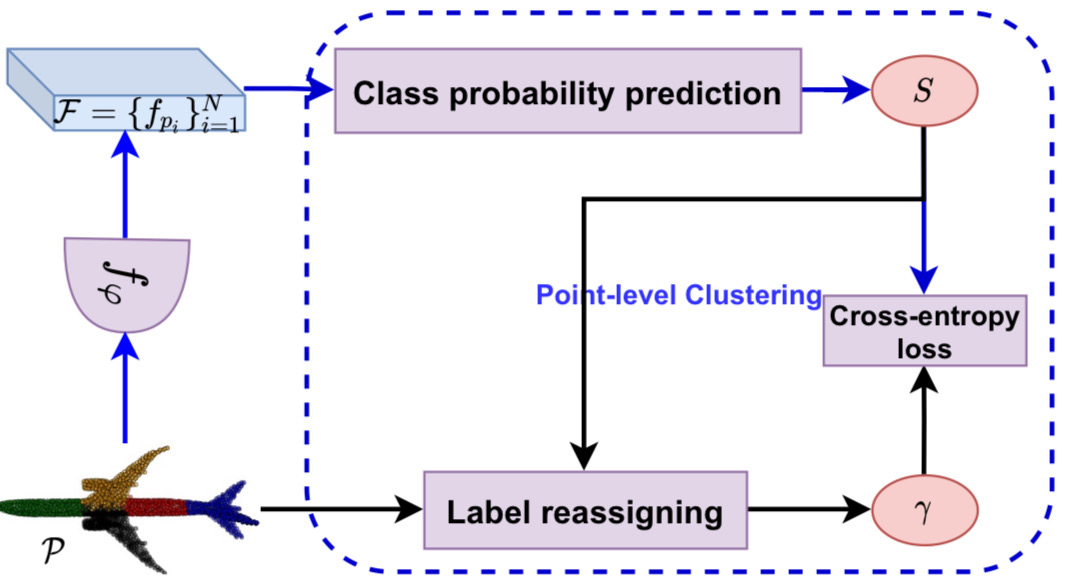
\includegraphics[width=300pt,height=180pt]{pictures/point_level.jpg}
    \caption{The architecture of the point-level clustering based unsupervised feature learning.\cite{mei2022unsupervised}}
    \label{fig:point_level}
\end{figure} 
 Now, the model already has the feature representation from the feature encoder backbone (eg. PointNet or  \ac{DGCNN}). The next step is the point-level clustering module. Fig.\ref{fig:point_level} gives a detailed visualization of the point-level clustering module. It can be seen that it is made up of 2 entities, the "class probability prediction" function and the "label reassigning". The point-level clustering module is analogous to the semantic segmentation task. Each point $p_i$ of the point cloud $\mathcal{P}$ is assigned to one of the $J$ predetermined possible subgroups or semantic categories. Essentially, it is achieved by processing each of the point cloud $\mathcal{\textbf{P}}$ followed by a point-level class probability prediction operator that yields a matrix for class probability $\mathit{\textbf{S}} = \{ s_{ij} \in [0,1]\}_{i,j}^{N,J}$. The label reassigning operator thus, takes the point cloud $\mathcal{\textbf{P}}$ and the class probability matrix $S$ and generates a pseudo-label matrix $\mathit{\mathbf{\gamma}} = \{ \gamma_{ij} \in \{0,1\}\}_{i,j}^{N,J}$. The weights for the encoder $f_{\varphi}$ are learnt such that it minimizes the average cross-entropy loss between the pseudo-label $\gamma$ and the predicted class probability $\textbf{S}$. The average cross entropy loss is calculated by the formula given in Eq.\ref{eq:avg_cross_entropy}.
\begin{equation}
    \label{eq:avg_cross_entropy}
    \mathit{H}(\gamma,\textbf{S})= \mathit{ - \frac{1}{N}} \langle \gamma,\log \textbf{S} \rangle = \mathit{ - \frac{1}{N}} \sum_{i=1}^{N} \sum_{j=1}^{J} \gamma_{ij} \log s_{ij}.
\end{equation}
But to train a network with a cross-entropy loss, the ground truth labels of the points in the point cloud are required. Since that is not available, one needs to assign the label $\gamma$ automatically, which is explained in details in the following passage. 

\subsubsection*{Class Probability Prediction}
As mentioned in the last passage, the output of the encoder $f_{\varphi}$ is fed as input to a classification head $\phi_\alpha$ and it generates a logit score for each of the feature vector as shown in Fig.\ref{fig:class_prob}. The vector for the logit score is given by $\textbf{g}_i = (g_{i1}, g_{i2},....., g_{iJ}), where \textbf{g}_i = \gamma_\alpha(f_{p_i})$. The classification head has 2 fully connected layers where each layer is a linear layer followed by a batch normalization. The leakyReLU activation function is used in all the layers except the last layer. As the output of the last layer N vectors for each of the N points in the point cloud is received where each of the output vector has $J$ dimensions, the number of predetermined subcategories each point cloud is to be segmented into. Thus, each entry of the feature vector is the probability of that point belonging to $j$-th category. Therefore, the logit score matrix $\textbf{G} = \{ g_{ij}\}_{i,j}^{N,J}$ has the dimension $N \times J$. The prediction that the point $p_i$ belongs to the category $j$ is computed by the application of a row-wise softmax operation on $\textbf{G}$ given by Eq.\ref{eq:softmax}.
\begin{equation}
    \label{eq:softmax}
    \mathit{s_{ij}}= \mathit{\frac{exp(g_{ij})}{\sum_{l=1}^{J}exp(g_{ij})}}. 
\end{equation}

\begin{figure}
    \centering
    \begin{minipage}[t]{.45\textwidth}
      \centering
      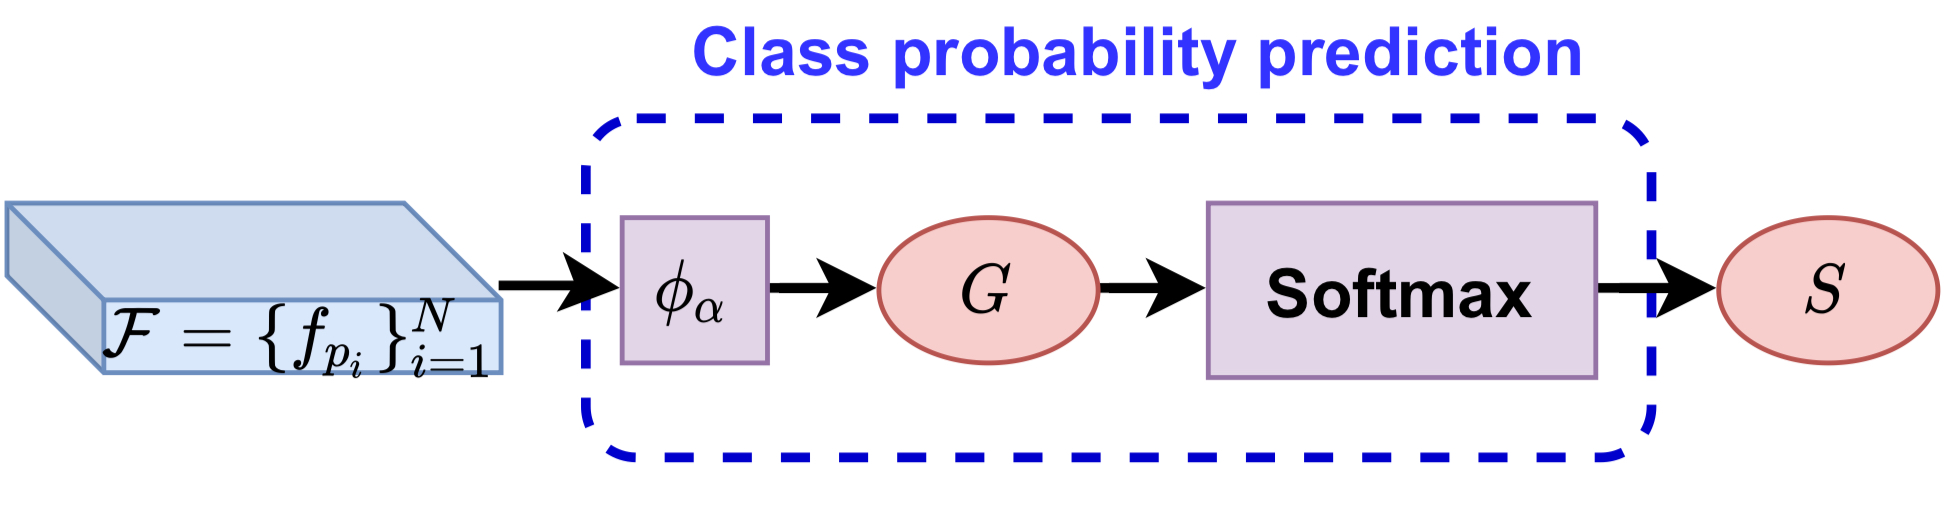
\includegraphics[width=200pt,height=100pt]{pictures/class_prob.jpg}
      \captionof{figure}{Architecture of class probability prediction.\cite{mei2022unsupervised}}
      \label{fig:class_prob}
    \end{minipage}%
    \hspace{1cm}
    \begin{minipage}[t]{.45\textwidth}
      \centering
      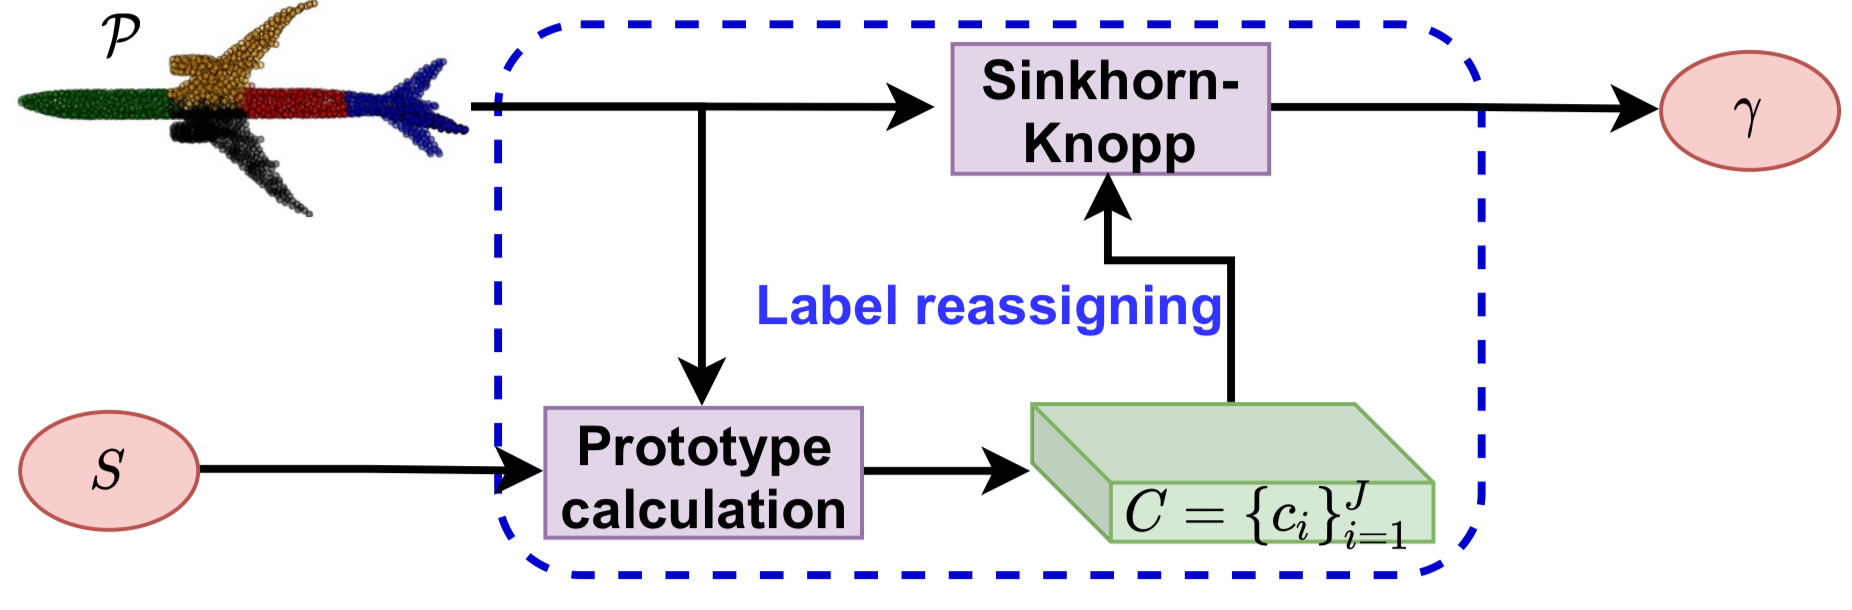
\includegraphics[width=200pt,height=100pt]{pictures/label_reassign.jpg}
      \captionof{figure}{Architecture of label reassigning \cite{mei2022unsupervised}}
      \label{fig:label_reassign}
    \end{minipage}
\end{figure}

\subsubsection*{Label reassigning}
In order to calculate the labels shown in Fig.\ref{fig:label_reassign}, the representative members of each of the semantic subgroups is needed. It can be done by selecting the cluster mean or cluster centers of each of these subgroups as the representative member of the cluster. The class probability matrix $S$ can be infered as the soft assignment of each point $p_i$ in the point cloud to $J$ semantic partitions. So the softly weighted mean of each of these partitions can be calculated as in Eq.\ref{eq:soft_mean}.

\begin{equation}
    \label{eq:soft_mean}
    \mathit{c_{j}}= \mathit{\frac{1}{\sum_{i=1}^{N}s_{ij}}\sum_{i=1}^{N}s_{ij}\mathbf{p}_i, j = 1,2,....,J}, 
\end{equation}
or in another way $C= \{c_j\}_{j_1}^J$ is a matrix with dimensions $J \times 3$. In a completely unsupervised learning setup, $\gamma \in [0,1]$ can be visualized as the posterior probability of a $p_i$ belong to the $j-th$ partition. $\gamma$ is optimized in the same method as in Eq.\ref{eq:softmax}. This results in a degenerate solution where each point is assigned to a single category. Thus, two assumptions are very pivotal for the reassigning of the labels. Firstly, the points in the point cloud ought to be partitioned into "equally-sized" partitions. In other words it can be formulated as $\mathit{\sum_{i=1}^{N}\gamma_{ij} = \frac{N}{J}}$. This is extremely importance in order to pretend all the points in the point cloud to be assigned to a single partition. Secondly, since the idea of using cluster centers as representative members of the partitions is inspired from the k-means algorithm, it means that if a point $p_i$ of the point cloud belongs to the $j^{*}$-th partition, the distance from $p_i$ to $c_j$ should be the shortest as compared to the distance of $p_i$ to all other cluster centers. In other words $ \lVert \mathbf{p}_i - c_{j^*} \rVert _2 \leq \lVert \mathbf{p}_i - c_{j} \rVert _2, j \neq j^* $. This is also equivalent to $ min_{\gamma}\sum_{i=1}^{N}\sum_{j=1}^{J} \gamma_{ij} \lVert \mathbf{p}_i - c_{j} \rVert _2^2$. This objective function is optimized to get $\gamma$. As per the rules of probability, the sum of all possible outcomes of an event is equal to 1, therefore $\sum_{j=1}^{J} \gamma_{ij} = 1$. Thus, the matrix of joint probability can be formulated as $\Gamma$ as $\Gamma = \frac{\gamma}{N}$ which has the elements $\Gamma_{ij} = \frac{\gamma_{ij}}{N}$. The distance matrix $\mathit{D = \{d_{ij}\}_{i,j}^{N,J}}$ has dimensions $\mathit{N \times J}$ where each element $\mathit{d_{ij}}$ is defined as $\mathit{d_{ij}} = \lVert \mathbf{p}_i - c_{j} \rVert _2^2$. In accordance to the assumptions stated above, the objective function $\mathit{D}$ could be minimized with respect to $\Gamma$ as in Eq.\ref{eq:label_reassign}.
\begin{equation}
    \label{eq:label_reassign}
    \begin{split}
        &\underset{\Gamma}{min \langle \Gamma, D \rangle},\\
        &s.t., \Gamma^{T}\vec{1}_{\mathit{N}} = \frac{1}{\mathit{J}}\vec{1}_{J} =, \Gamma\vec{1}_{J} = \frac{1}{\mathit{N}}\vec{1}_{\mathit{N}},
    \end{split}    
\end{equation}
where $\vec{1}_{J}$ is the vector of ones having dimension $J$. The above condition enforces that each of the cluster representative is  selected atleast $\frac{N}{J}$ times for each point cloud and $\sum_{j=1}^{J}\gamma_{ij}=1$. The objective function as defined in Eq.\ref{eq:label_reassign} is a typical case of an optimal transport problem \cite{peyre2019computational}. Such problems can be solved by the Sinkhorn-Knopp algorithm \cite{cuturi2013sinkhorn}. In other words, it means solving the entropic regularized objective function in Eq. \ref{eq:entropy_regular}.
\begin{equation}
    \label{eq:entropy_regular}
    \begin{split}
        &\underset{\Gamma}{min \langle \Gamma, D \rangle} - \lambda \mathit{H}(\Gamma),\\
        &s.t., \Gamma^{T}\vec{1}_{\mathit{N}} = \frac{1}{\mathit{J}}\vec{1}_{J} =, \Gamma\vec{1}_{J} = \frac{1}{\mathit{N}}\vec{1}_{\mathit{N}},
    \end{split}    
\end{equation}
where, $\mathit{H}(\Gamma) = \langle \Gamma, \log \Gamma -1 \rangle $ is the entropy of $\Gamma$ and $\lambda$ is the regularization parameter. As per \cite{cuturi2013sinkhorn}, on solving Eq. \ref{eq:entropy_regular}, the normalized exponential matrix in Eq. \ref{eq:gamma} is attained. 
\begin{equation}
    \label{eq:gamma}
    \Gamma = diag(\mu) exp(\mathit{D/\lambda}) diag(\nu),
\end{equation}
where $\mu$ and $\nu$ are renormalized vectors in $\mathbb{R}^N$ and $\mathbb{R}^J$ respectively and $exp()$ is the exponential function. These vectors are computed on utilizing the iterative Sinkhorn-Knopp algorithm\cite{cuturi2013sinkhorn} with the constraints $ \mu = \frac{1}{\mathit{N}} \vec{1}_{\mathit{N}} $ and $ \nu = \frac{1}{\mathit{J}} \vec{1}_{\mathit{J}} $. The pseudo-code for the Sinkhorn-Knopp algorithm is elaborated in Algorithm \ref{alg:sinkhorn}.

\begin{algorithm}[h]
    \caption{Pseudo-code for Sinkhorn-Knopp algorithm}\label{alg:sinkhorn}
    def sinkhorn($D, \epsilon, niters=3$)
    \begin{algorithmic}[1]
        \State $\Gamma = exp(D/ \epsilon)^T$
        \State $\gamma /= sum(\Gamma)$
        \State $N, J = \Gamma .shape$
        \State $u,r,c = zeros(N), ones(J)/J, ones(N)/N$
        \For{$\; in range (0, \; niters)$}
            \State $u = sum(\Gamma, dim=1)$
            \State $\Gamma *= (r/u).unsqueeze(1)$
            \State $\Gamma *= (c/sum(\Gamma, dim=0)).unsqueeze(0)$            
        \EndFor
        \State $\mathbf{return} \; \Gamma$          
    \end{algorithmic}
\end{algorithm}

Thus, the overall point-level clustering can be encapsulated by an \ac{EM} like algorithm. The network learns the parameters $f_{\varphi}$ and $\mathcal{\phi}_{\alpha}$ by optimization of Eq.\ref{eq:avg_cross_entropy} and get a label reassigning matrix $\gamma$ by solving the optimization problem in Eq. \ref{eq:gamma} with respect to $\Gamma$. It is executed by performing the following steps in repetition. 
\begin{itemize}
    \item Step 1: representation learning. Having the current probability matrix $\gamma$, the weights of the model are updated by optimizing Eq. \ref{eq:avg_cross_entropy} with respect to the  parameters $f_{\varphi}$ and $\mathcal{\phi}_{\alpha}$. It is in line with the supervised case where the model uses the cross entropy loss for classification. 
    \item Step 2: label reassigning. On having the updated set of $f_{\varphi}$ and $\mathcal{\phi}_{\alpha}$, $\Gamma$ is calculated by using Eq. \ref{eq:gamma}. The posterior probability matrix is then computed by $\gamma = \mathit{N} \cdot \Gamma$.
\end{itemize}
Thus, each update step requires a single matrix-vector multiplication which has the time complexity of $O(\mathit{N \times J})$ which means the computation time increases linearly with the increase in the number of points in the point cloud. Therefore, scalability of this method is quite high and the process remains relatively quick even for a million samples in the dataset. Moreover, the orthogonal regularization is introduced to circumvent the issue of having the same output vector for all cluster representatives. It is computed by 
\begin{equation}
    \label{eq:orth}
    \mathcal{L}_{\mathit{orth}}(\mathit{C}) = \lVert \mathit{C_{*}^{T} C_{*} - I} \rVert _{1},
\end{equation}
where $ \lVert \cdot \rVert _1 $ is the $l_{1}$-norm or the Manhattan distance and $\mathit{C_{*}} = [ \frac{c_1}{\lVert c_1 \rVert _{2}}, \frac{c_2}{\lVert c_2 \rVert _{2}}, ... , \frac{c_{\mathit{J}}}{\lVert c_{\mathit{J}} \rVert _{2}}]$. The pseudo-code for the point-level clustering module in elaborated in Alg. \ref{alg:point_level}.

\begin{algorithm}[H]
    \caption{Pseudo-code for point-level clustering}\label{alg:point_level}
    \textbf{Input:} $\{\mathcal{P}\}$: is a set of 3D point clouds with $\mathit{N}$ number of points in it; $\mathit{K}$: number of epochs. \\
    \textbf{Output:} backbone $f_{\varphi}$.
    \begin{algorithmic}[1]
        \For{$i$ in range $(0,K)$}
            \State $\mathcal{L} = 0$
            \For{$\mathcal{P} \in \{\mathcal{P}\}$}
                \State \# Computes Class probability
                \State $ S = softmax(\phi_{\alpha}(f_{\varphi}(\mathcal{P})))$
                \State \# Computes cluster representatives of partitions
                \State $ C = \left\{ \frac{1}{\sum_{i=1}^{N}s_{ij}} \sum_{i=1}^{N}s_{ij}\mathbf{p}_i \right\}_{j=1}^N$
                \State \# Computes mean-squared error 
                \State $ D = \left\{ \lVert \mathbf{p}_i - c_j \rVert _2^2 \right\} _{i,j}^{N,J}$
                \State \# Computes posterior probability matrix
                \State $\gamma = sinkhorn(\ac{stop-grad}(D), 1e - 3, 20)$
                \State \# Computes Loss Function 
                \State $\mathcal{L} = H(\gamma,S) + \eta \mathcal{L}_{orth}(C)$
            \EndFor
            \State \# Updates backbone, projector ad predictor
            \State $ f_{\varphi}, \phi_{\alpha} \gets optimize(\frac{\mathcal{L}}{N})$
        \EndFor
        \State $\mathbf{return \; f_{\varphi}}$          
    \end{algorithmic}
\end{algorithm}

\subsubsection{Instance-Level Contrasting Module}
\begin{figure}[t]
    \centering
    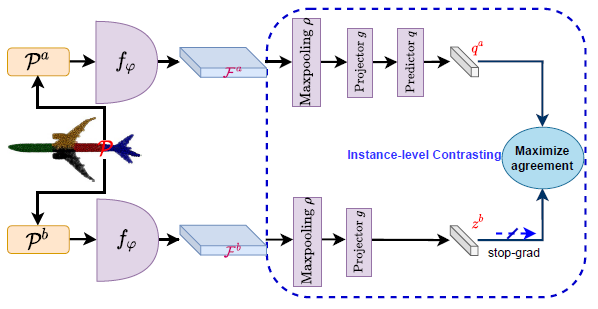
\includegraphics[width=300pt,height=180pt]{pictures/ConClu.png}
    \caption{The architecture of the instance-level Contrasting.\cite{mei2022unsupervised}}
    \label{fig:global_level}
\end{figure} 
This module plays a crucial role in learning the global features of the point clouds. The architecture of this module is shown in Fig. \ref{fig:global_level}. The network is fed with two augmented views $\mathcal{P}^a$, $\mathcal{P}^b$ of the same point cloud $\mathcal{P}$. The feature representation obtained as the output of the encoder backbone $f_{\varphi}$, are fed to a MaxPooling layer $\rho$, the output of which is fed to a projection \ac{MLP} head $g$ \cite{chen2021exploring}. The encoder backbone $f_{\varphi}$ and the projection head $g$ shares the weights for both the augmented views. The output of the projection head of one of the augmented views (the top branch) is fed to the prediction head $q$. The purpose of this unit is to transform the output of one of the augmented views to match the other. The operation is applied to only one augmented view to make the network asymmetric \cite{grill2020bootstrap}. In other words, the output vectors can be realized as  $ \mathit{q^a} \triangleq \mathit{\mathbf{q}(g(\rho(\mathbf{\mathcal{F}}^a)))}$ and $\mathit{\mathbf{z}^b} \triangleq \mathit{g(\rho(\mathbf{\mathcal{F}}^b))}$ where $\mathbf{\mathcal{F}}^a = f_{\phi}(\mathbf{\mathcal{P}}^a)$ and $\mathbf{\mathcal{F}}^b = f_{\phi}(\mathbf{\mathcal{P}}^b)$. Keeping in line with \cite{chen2021exploring}, \ac{stop-grad} is applied on the second branch $z^b$ to resist the network from generating a constant mapping without using negative samples for contrastive learning. The network is constructed such that the similarity between $\mathit{q^a}$ and $\mathit{z^b}$ is maximized. Mathematically speaking, the mean-squared error between the $\mathit{l}_2$-normalized prediction $q^a$ and projection $\mathit{z_b}$ is minimized as shown in Eq. \ref{eq:error}. 
\begin{equation}
    \label{eq:error}
    \mathcal{D}(\mathit{q^a, z^b}) \triangleq \lVert \frac{\mathit{q^a}}{\lVert \mathit{q^a} \rVert _2} - \frac{\mathit{z^b}}{\lVert \mathit{z^b} \rVert _2} \rVert _2^2 = 2 - \frac{2\mathit{q^{aT}z^b}}{\lVert q^a \rVert _2 \cdot \lVert z^b \rVert _2}.
\end{equation}

In other words, it is the negative cosine similarity, up to a scale of 2. Since, \ac{stop-grad} is enforced on $z^b$, Eq. \ref{eq:error} is modified by the following Eq. \ref{eq:error_stop-grad}.
\begin{equation}
    \label{eq:error_stop-grad}
    \mathcal{D}(\mathit{q^a, \ac{stop-grad}(z^b)}), 
\end{equation}
which means $z^b$ acts as a constant vector in this equation. Keeping in line with \cite{chen2021exploring}, a global symmetrized loss is defined as in Eq. \ref{eq:sym_loss}.
\begin{equation}
    \label{eq:sym_loss}
    \mathcal{L}_{\mathit{global}} = \mathcal{D}(\mathit{q^a, \ac{stop-grad}(z^b)})  + \mathcal{D}(\mathit{q^b, \ac{stop-grad}(z^a)}). 
\end{equation}
The minimum value the above equation can attain is 0. This is because, in the first term of the equation, the encoder backbone $q^a$ gets no gradient flow from $z^b$. But it gets gradients from $q^b$ in the second term. In the same way, in the second term of the equation, the encoder backbone $q^b$ gets no gradient flow from $z^a$. But it gets gradients from $q^a$ in the first term. if the \ac{stop-grad} mechanism is not applied, then in spite of having a loss of zero during training, the representations learnt by the network would be futile i.e. all the point clouds would be mapped to the same feature representation. Or in other words, the network would crumble to  constant mapping \cite{chen2021exploring}. The pseudo-code for this module is shown in Alg. \ref{alg:instance_level}.

\begin{algorithm}[H]
    \caption{Pseudo-code for instance-level clustering}\label{alg:instance_level}
    \textbf{Input:} $\{\mathcal{P}\}$: is a set of 3D point clouds with $\mathit{N}$ number of points in it; $\mathit{K}$: number of epochs. \\
    \textbf{Output:} backbone $f_{\varphi}$.
    \begin{algorithmic}[1]
        \For{$i$ in range $(0,K)$}
            \State $\mathcal{L} = 0$
            \For{$\mathcal{P} \in \{\mathcal{P}\}$}
                \State \# Generate random augmentations
                \State $ \mathcal{P}^a = aug(\mathcal{P})$
                \State $ \mathcal{P}^b = aug(\mathcal{P})$
                \State \# Compute projections
                \State $\mathit{z^a = g(\rho(f_{\varphi}(\mathcal{P}^a)))}$
                \State $\mathit{z^b = g(\rho(f_{\varphi}(\mathcal{P}^b)))}$
                \State \# Compute predictions
                \State $\mathit{q^a, q^b = q(z^a), q(z^b)}$
                \State \# Calculate loss
                \State $\mathcal{L} += \mathcal{D}(\mathit{q^a, \ac{stop-grad}(z^b)})  + \mathcal{D}(\mathit{q^b, \ac{stop-grad}(z^a)})$
            \EndFor
            \State \# Updates backbone, projector ad predictor
            \State $ f_{\varphi}, g, q \gets optimize(\frac{\mathcal{L}}{N})$
        \EndFor
        \State $\mathbf{return \; f_{\varphi}}$          
    \end{algorithmic}
\end{algorithm}

\subsubsection{Loss Function}
The objective of the network is to simultaneously minimize both the point-level clustering loss and the instance level contrasting loss. If the two augmented views of the point cloud $\mathcal{P}$ are $\mathcal{P}^a$ and $\mathcal{P}^b$, then the point-level clustering loss can be calculated by Eq. \ref{eq:local_loss}.
\begin{equation}
    \label{eq:local_loss}
    \mathcal{L}_{\mathit{local}} = H(\gamma^{a}, S^a) + H(\gamma^{b}, S^b) + \eta(\mathcal{L}_{orth}(C^a) + \mathcal{L}_{orth}(C^b))
\end{equation}
where $\eta>0$ is a regularization parameter. Here $\gamma^a$ is the posterior class probability of the point belonging to one of the subcategories, $S^a$ is the predicted class probability and $C^a$ is the normalized center of the augmented view of the point cloud $\mathcal{P}^a$. In the same way, the corresponding terms for the other augmented view $\mathcal{P}^b$ are $\gamma^b$, $S^b$ and $C^b$. Therefore, the total loss could be calculated as the linear combination of $\mathcal{L}^{global}$ and $\mathcal{L}^{local}$ as in Eq. \ref{eq:total_loss}.
\begin{equation}
    \label{eq:total_loss}
    \mathcal{L}_{\mathit{total}} = \mathcal{L}_{\mathit{local}} + \mathcal{L}_{\mathit{global}}.
\end{equation}

\subsection{Dimensionality Reduction}
\subsubsection{Reasons for Dimension Reduction}
The goal of this thesis is to find a diverse set of objects that collectively represent the entire ABC dataset \cite{Koch_2019_CVPR}. This set of objects is to be then used as the source library for the different transfer learning approaches to be used in bin picking applications. Therefore, clustering algorithms are necessary to find the representative members of the dataset. In order to facilitate the usage of the \ac{DBCV} Index as the evaluation metric for the clustering algorithm as mentioned in Ch. \ref{sec:dbcv}, it is necessary to reduce the dimensions of the latent space representations. Furthermore, it would be beneficial to find lesser but denser clusters. This means that fewer objects could collectively represent the entire dataset and each representative member would be similar to a greater number of other objects in the dataset. Thus, reducing the dimensions of the latent space representations by dimensionality reduction would entail more "crowded" clusters in case of density-based clustering algorithms.

\subsubsection{T-distributed Stochastic Neighbor Embedding}
A technique for reducing dimensionality, \ac{t-SNE} is mostly used for data visualization in 2D and 3D maps. This approach has become well-liked since it can identify non-linear relationships in the data. If the data has more than two or three features, it might be necessary to consider looking for clusters in the data. To better understand the data and determine how many clusters to use in clustering models like k-means, if necessary. To further grasp what one hopes to obtain, the following example is used for illustration. It is assumed that the data is to be converted from a 2D space to a 1D dimension as shown in Fig. \ref{fig:2d_data} and Fig. \ref{fig:1d_data} respectively.\cite{van2008visualizing}

\begin{figure}
    \centering
    \begin{minipage}[t]{.45\textwidth}
      \centering
      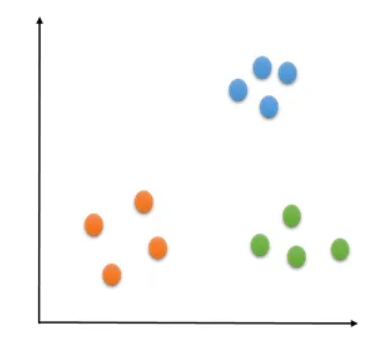
\includegraphics[width=150pt,height=120pt]{pictures/2d_data.PNG}
      \captionof{figure}{The original data in 2-D space \cite{tsne}.}
      \label{fig:2d_data}
    \end{minipage}%
    \hspace{5mm}
    \begin{minipage}[t]{.45\textwidth}
      \centering
      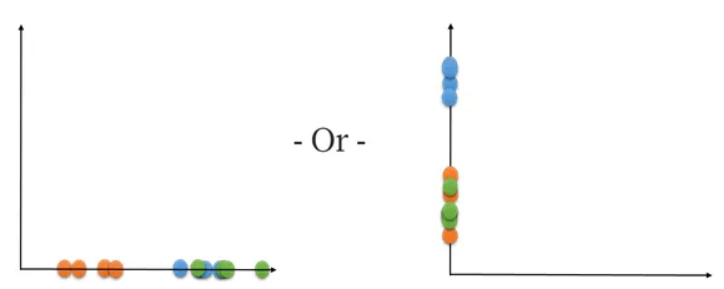
\includegraphics[width=200pt,height=120pt]{pictures/1d_data.PNG}
      \captionof{figure}{Data projected to 1-D space \cite{tsne}.}
      \label{fig:1d_data}
    \end{minipage}  
\end{figure}
Every color in this illustration denotes a cluster. It is evident that the densities of each cluster differ. It can be observed that at least two of the clusters overlap when a simple projection of the data onto one of its dimensions is performed. This highlights that a better method is necessary for the dimension reduction task. This problem is handled by the \ac{t-SNE} algorithm and its effectiveness is described in the following steps.
\begin{itemize}
    \item Determining a joint probability distribution that captures the commonalities amongst the data points.\cite{van2008visualizing}
    \item Constructing a dataset of the points with the target dimension and thereafter computing the joint probability distribution of those points as well.\cite{van2008visualizing}
    \item Gradient descent is used to transform the low-dimensional dataset into a joint probability distribution that is as close as feasible to the high-dimensional dataset.\cite{van2008visualizing}
\end{itemize}

\vspace{5mm}

\textbf{Working principle of \ac{t-SNE}}\\
\begin{enumerate}
    \item \textbf{The likelihood of points to belong to the same neighborhood}\\
    Finding each point's Euclidean distance from every other point is the initial step in the process. Next, these distances are converted into conditional probabilities, which express how similar one pair of points is to the other. This means that it is required to determine the degree of similarity—that is the likelihood—between any two points in the data. A Gaussian distribution with a standard deviation of $\sigma_i$ and a center at $x_i$ represents the conditional probability of point $x_j$ to be next to point $x_i$. The conditional probability is defined mathematically as shown in Eq. \ref{eq:cond_prob}. The factors that effect $\sigma_i$ are discussed later.
    \begin{equation}
        \label{eq:cond_prob}
        \mathit{p_{j|i}} = \mathit{\frac{exp \left(- \frac{\lVert x_i - x_j \rVert ^2}{2 \sigma_i^2} \right)}{\sum_{k \neq i} exp \left(- \frac{\lVert x_i - x_k \rVert ^2}{2 \sigma_i^2} \right)}}, 
    \end{equation}
    where $p_{j|i}$ is the probability that the point $x_i$ has $x_j$ as its neighbor. Since the clusters can have varying densities, the division by the total of all the other points positioned at the Gaussian distribution centered at $x_i$ is necessary. Looking back to Fig. \ref{fig:2d_data} as an example to clarify, the orange cluster has a lesser density than the blue. As a result, there will be less similarity between the orange and blue points if the Gaussian distribution is used to compute the commonalities between each pair of points. The normalization is performed because it is only necessary to view the clusters as such in the final output and if any of the clusters have differing densities need not be visualized. The joint probability distribution can be computed from the conditional distributions as shown in Eq. \ref{eq:joint_prob}.\cite{van2008visualizing}
    \begin{equation}
        \label{eq:joint_prob}
        \mathit{p_{ij}} = \mathit{\frac{p_{j|i} + p_{i|j}}{2n}}. 
    \end{equation}
    One of the ways that the t-SNE approach differs from the previous SNE is that it uses the joint probability distribution instead of the conditional probability. The computation in the third stage of the algorithm is made simpler by the symmetric property of the pairwise similarities $(p_{ij} = p_{ji})$.
    \item \textbf{Transformation of the data to a lower dimension}\\
    In this step, a joint probability distribution for the points in the low-dimensional space is computed. In order to achieve that, a new dataset is created at random that has K features (K being the desired dimension) and the same amount of points as the original dataset. As the dimension reduction is performed for visualization, K will often be two or three. Returning to the example, the \ac{t-SNE} algorithm now creates a random dataset of 1D points as shown in Fig. \ref{fig:random_1d_data}.
    \begin{figure}
        \centering
        \begin{minipage}[t]{.45\textwidth}
          \centering
          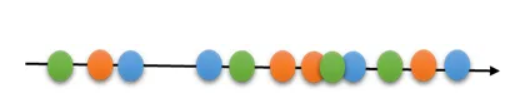
\includegraphics[width=150pt,height=50pt]{pictures/random_1d_data.PNG}
          \captionof{figure}{A random dataset created in 1D space \cite{tsne}.}
          \label{fig:random_1d_data}
        \end{minipage}%
        \hspace{5mm}
        \begin{minipage}[t]{.45\textwidth}
          \centering
          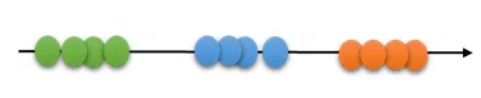
\includegraphics[width=150pt,height=50pt]{pictures/tsne_output.PNG}
          \captionof{figure}{Visualization of the dataset in 1D space after applying \ac{t-SNE} \cite{tsne}.}
          \label{fig:tsne_output}
        \end{minipage}  
    \end{figure}
    Similar to the original dataset, the joint probability distribution for this set of points is generated using the t-distribution rather than the Gaussian distribution. The points in this case are denoted as $y$ and the probabilities as $q$ and thus, the joint probability distribution is computed as shown in Eq. \ref{eq:joint_prob_random}.
    \begin{equation}
        \label{eq:joint_prob_random}
        \mathit{q_{ij}} = \frac{\left(1 + \lVert y_i - y_j \rVert\right) ^{-1}}{\sum_{k \neq l}\left(1 + \lVert y_k - y_l \rVert\right) ^{-1}}.
    \end{equation}
    The heavy tails attribute of the t-distribution is the rationale behind selecting it over the Gaussian distribution. This property helps minimize "crowding" of the points in the lower dimension by making moderate gaps between points in the high-dimensional space. An additional benefit of employing the t-distribution is that it enhances the algorithm's optimization procedure in the third stage.\cite{van2008visualizing}
    \item \textbf{Modification of the dataset in the low-dimensional space for the best possible data visualization}\\
    Now, the \ac{KL} divergence is utilized to maximize the similarity between the joint probability distribution of the data points in the low dimensional space and the higher dimensional space. The \ac{KL} divergence serves as a gauge for the degree of difference between two distributions. It is defined for distributions P and Q in the probability space of $\chi$ by Eq. \ref{eq:kl_div}.
    \begin{equation}
        \label{eq:kl_div}
        \mathit{D}_{\ac{KL}}(\mathit{P} || \mathit{Q}) = \sum_{x \in \chi} \mathit{P(x)} \log \left( \frac{\mathit{P(x)}}{\mathit{Q(x)}} \right).
    \end{equation}
    In instances where the distributions are identical, the KL divergence value approaches to 0, indicating an increase in similarity between the distributions. The lower dimension dataset is modified so that, in the joint probability distribution, it resembles the original data as soon as possible. To do this, gradient descent is used. The KL divergence between the joint probability distributions P from the high-dimensional space and Q from the low-dimensional space is the cost function that the gradient descent algorithm seeks to minimize as defined in Eq. \ref{eq:kl_div_cost}.
    \begin{equation}
        \label{eq:kl_div_cost}
        \mathit{C} = \mathit{\ac{KL}(P || Q)} = \sum_i \sum_j \mathit{p_{ij}} \log \mathit{\frac{p_{ij}}{q_{ij}}}.
    \end{equation}
    The low dimension dataset's point values are obtained from this optimization, which is then utilized for visualizing the dataset in the lower dimensional space. Refering to the example before, the clusters in the low-dimensional space appears as in Fig. \ref{fig:tsne_output}. The \ac{t-SNE} model has a number of hyperparameters that can be fine-tuned depending on the use-case. A few of these have to do with gradient descent. The two most crucial ones are the number of iterations, the learning rate and perplexity. It serves to select the Gaussian distribution expressing the conditional distribution in high-dimensional space's standard deviation $\sigma_i$. It can be defined as the count of each point's effective neighbors. For perplexities ranging from 5 to 50, the model is fairly robust.\cite{van2008visualizing}

\end{enumerate}

\subsection{Clustering Algorithms}

\subsubsection{Requirements and Conditions}
\label{sec:clustering_algo}
Once the feature representations are obtained, multiple clustering algorithms are utilized to group the objects in the datasets into clusters. For this, one algorithm from each type of clustering algorithms as mentioned in \ref{sec:Clustering_Algorithms} are implemented to analyze the behavior of different clustering algorithms in this use case. Since the ultimate goal of the task in hand is to find representative members of the dataset, it is more robust to find the medoid of the cluster instead of the arithmetic mean. As mentioned in \ref{sec:Distribution_based_Clustering}, the medoids are actual datapoints of the dataset which is more practical to use in this use case instead of using a rather blurred, noisy arithmetic mean of the clusters. 

\subsubsection{Selected Clustering Algorithms}
The scikit-learn implementations of the k-medoids algorithm \cite{scikit_learn_kmedoids}, spectral clustering algorithm \cite{scikit-learn} and agglomerative clustering algorithm \cite{scikit-learn} are used for this purpose. Since the spectral clustering algorithm and agglomerative clustering algorithm implementations provide the cluster centres and not the cluster medoids at the end, an additional step is necessary to compute the cluster medoids. Another clustering algorithm that is suggested for this task is the "multi-level \ac{HDBSCAN}" clustering. The traditional implementation of the \ac{HDBSCAN} algorithm available in scikit-learn can provide hierarchical density based clusters. However, this algorithm does not provide any control on the number of clusters that can be generated. Thus, in the presence of very large datasets like the ABC \cite{Koch_2019_CVPR} dataset, it can potentially generate more than a hundred thousand clusters and thus, that many number of cluster representative members. Generating that many data for the source library in the current infrastructure present at \ac{IPA} is extremely computationally expensive and thus, technically infeasible. Increasing the minimum cluster size to be considered as a cluster and increasing the minimum number of samples around a point to be considered as a core point can decrease the overall number of cluster but that would also mean that the algorithm would label more datapoints as outliers. Losing too much information about the objects as outliers can jeopardize the purpose of a source library which is expected to generalize the feature of maximum possible objects in the dataset. 

\vspace{5mm}

\textbf{Working principle of multi-level \ac{HDBSCAN} algorithm}
\begin{enumerate}
    \item At first \ac{HDBSCAN} algorithm is applied on the whole dataset. After the clustering algorithm, $p$ medoids are obtained. These $p$ datapoints are the relevant points for the next step.
    \item The \ac{HDBSCAN} algorithm is applied again on those $p$ datapoints. As a result of it, $m$ clusters are obtained and $n$ datapoints are labelled as outliers. Thus, there would be $m$ medoids which are the representative members of each of the clusters. From this level onwards, no new datapoints would be discarded as outliers. Thus, each of the datapoints labelled as outliers would be assigned to a new cluster along with all the fellow cluster member which is a part of the cluster this particular datapoint is a member of in the previous level. The pseudo-code for this part of the algorithm is shown in Alg. \ref{alg:multi_level_hdbscan}. 
    \item Thus, the relevant datapoints for the next level are the $m$ medoids and all the $n$ outliers relabelled as medoids of new clusters. Step 2 and 3 are repeated until convergence, i.e. when $m + n \leq k$ where $k$ is the maximum number of permissible clusters as shown in Alg. \ref{alg:hier_cluster}.
\end{enumerate}
After the convergence of the algorithm, $c$ medoid points are obtained which are the representative members of the $c$ clusters where $c \leq k$. Similar to the k-medoids algorithm, the Euclidean distance metric is used to compute the medoids. The $"min\_cluster\_size"$ hyperparameter controls the minimum number of datapoints to be contained in a cluster. Increasing this value would mean clusters with more number of elements. But this would also mean that groups smaller than this size would be treated as outliers. Thus, increasing this value could lead to significant loss of information about the features of different objects in the cluster. To circumvent this issue, the value of this parameter is kept at its default value which is 2. This is the reason why \ac{HDBSCAN} algorithm returns a significantly high number of clusters. Thus, the proposal of multi-level \ac{HDBSCAN} algorithm is deemed necessary for this use case.

\begin{algorithm}[H]
    \caption{Pseudo-code for hierarchical clustering}\label{alg:hier_cluster}
    \textbf{Input:} $\{\mathcal{E}\}$: is the set of feature representations for all objects in the dataset, $K$ is the number of permissible clusters.\\
    \textbf{Output:} $\{\mathcal{P}_R\}$ is the set of representative members of the dataset.
    \begin{algorithmic}[1] 
        \State $\mathcal{E}_R \leftarrow \{\mathcal{E}\}$               
        \State $classifier,\; predictions,\; num\_clusters = \ac{HDBSCAN}(\mathcal{E}_R)$
        \State $count \leftarrow 0$
        \State $C \leftarrow predictions$
        \State $cluster\_members = get\_cluster\_members(C, \{\mathcal{E}\})$
        \State $clusters = list(unique(C))$
        
        \While{$True$}
            \State $\mathcal{E}_R, \; C, \; cluster\_members, \; num\_clusters \; classifier = get\_hier\_clusters(\mathcal{E}, \; \mathcal{E}_R, \; C, \; cluster\_members, count)$
            \State $count +=1$
            \State $total\_num\_clusters = len(list(unique(C)))$
            \If{$total\_num\_clusters \leq K \; \mathbf{or} \; n\_clusters \; is \; 0$}
                \State break
            \EndIf            
        \EndWhile
        \State $medoid\_indices = get\_medoid\_indices(\mathcal{E}_R, \mathcal{E}\ )$
        \State $\{\mathcal{P}_R\} = \{\mathcal{P}_i, \; \mathcal{P}_i \in \{\mathcal{P}\} \; and \; i \in medoid\_indices\}$
        \State $\mathbf{return \;}\{\mathcal{P}_R\}$          
    \end{algorithmic}
\end{algorithm}

\begin{algorithm}[H]
    \caption{Pseudo-code for multi-level \ac{HDBSCAN} clustering}\label{alg:multi_level_hdbscan}
    \textbf{Input:} $\{\mathcal{P}\}$: is a set of 3D point clouds with $\mathit{N}$ number of points in it, $\{\mathcal{E}\}$: is the set of feature representations for all objects in the dataset, $\{\mathcal{E}_R\}$ is the set of feature representations for relevant points objects in the dataset, $C$ is the cluster membership of all the points clouds in the dataset, $clusters$ is the list of all clusters, $clusters\_members$ is the list of all the point clouds in the dataset, grouped by their cluster membership, $count$ is the current level of multi-level \ac{HDBSCAN}\\
    \textbf{Output:} $\mathcal{E}_R, \; C, \; cluster\_members, \; num\_clusters, \; classifier$ 
    \begin{algorithmic}[1] 
        \State $classifier,\; predictions,\; num\_clusters = \ac{HDBSCAN}(\mathcal{E}_R)$
        \State $medoids = classifier.medoids$
        \State $cluster\_pointer \leftarrow num\_clusters$
        \State Assign Empty list to $outlier\_list$
        \For{$\forall \; obj\_idx, \, object \in enumerate(\mathcal{E}_R)$}
            \If{$prediction[obj\_idx] < 0$}
                \State $AddItem(outlier\_list, \; obj\_idx)$
                \State $C[cluster\_members[obj\_idx]] = cluster\_pointer$
            \Else
                \State $C[cluster\_members[obj\_idx]] = prediction[obj\_idx]$
            \EndIf
        \EndFor
        \State $\{\mathcal{O}\} = \{\mathcal{E}_i, \; \mathcal{P}_i \in \{\mathcal{E}_R\} \; and \; i \in outlier\_list\}$
        \State $cluster\_members = get\_cluster\_members(C,\{\mathcal{E}\})$
        \State $medoid\_indices = get\_medoid\_indices(medoids, \mathcal{E}_R\ )$
        \State $\mathcal{E}_R = \{\mathcal{E}_i, \; \mathcal{E}_i \in \{\mathcal{E}_R\} \; and \; i \in medoid\_indices\}$
        \If{$count \neq 0$}
            \State $\mathcal{E}_R = concatenate(\mathcal{E}_R, \; \mathcal{O})$
        \EndIf
        \If{$count \; is \; 0$}
            \State $num\_clusters = len(list(unique(C)))$
        \EndIf
        \State $\mathbf{return \;}\mathcal{E}_R, \; C, \; cluster\_members, \; num\_clusters, \; classifier$ 
    \end{algorithmic}
\end{algorithm}

 The \ac{HDBSCAN} algorithm performs the \ac{DBSCAN} algorithm for different epsilon values and hence provides a more robust clustering algorithm. Moreover, the optimum value of epsilon is case-dependent and no single value is suitable for clustering different datasets. This also means that expert domain knowledge is essential for determining the optimum epsilon value and is difficult to obtain in this use case. Thus, it is logical to use the \ac{HDBSCAN} algorithm in this use case as it incorporates the result of clustering for different epsilon value and finds the clustering solution that provides the optimum stability over all epsilon. The \ac{HDBSCAN} algorithm can opt for different algorithms like \ac{KD}-trees, Ball Tree or brute-force algorithm. 

\vspace{5mm}

\textbf{\ac{KD}-tree algorithm}
The \ac{KD}-tree is a data structure that is used for the purpose of effectively organizing and searching for points in multi-dimensional spaces. Specifically, \ac{KD}-trees excel at solving the nearest neighbor search problem, which involves finding the closest data points to a given query point. The structure of a \ac{KD}-Tree resembles a binary tree, where each node can have up to two children. It operates by recursively dividing data points along different dimensions, creating a hierarchical arrangement that facilitates efficient search and retrieval as shown in Fig. \ref{fig:kd_tree}. 
\begin{figure}[t]
    \centering
    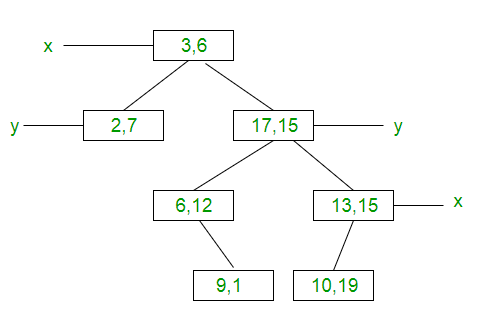
\includegraphics[width=300pt,height=180pt]{pictures/ktree_1.png}
    \caption{A demonstration of the \ac{KD}-tree algorithm with 7 datapoints having 2 dimensions x and y.\cite{kd_tree}}
    \label{fig:kd_tree}
\end{figure} 
At each level, the tree selects a dimension and splits the data points into two groups based on their values in that dimension. This process continues until all data points are assigned to leaf nodes. One of the key advantages of \ac{KD}-Trees lies in their ability to handle high-dimensional data in static dataset—a common challenge in machine learning applications like computer vision, natural language processing and bioinformatics. High-dimensional data often suffers from the “curse of dimensionality,” where the search space grows exponentially with the number of dimensions, making nearest neighbor queries time-consuming. As the ABC \cite{Koch_2019_CVPR} dataset is an immensely high dimensional dataset, the \ac{KD}-Tree algorithm is used in this use case. \ac{KD}-Trees address this by narrowing down the search space at each tree level, resulting in faster queries. Despite their advantages, \ac{KD}-Trees face limitations and challenges. One concern arises when the number of dimensions increases, particularly with non-uniformly distributed data points. In such cases, the tree may become unbalanced, resulting in inefficient search times. But since the datapoints are reduced to 2-dimensional datapoints, the \ac{HDBSCAN} algorithm doesn't result to inefficient search times in this case. Also \ac{KD}-trees are sensitive to outliers. The steps for \ac{KD}-tree algorithm are:
\begin{enumerate}
    \item \textbf{Dimension Selection}: A dimension is chosen along which the data is split \cite{friedman1975algorithm}.
    \item \textbf{Sorting}: The data points are sorted and arranged.
    \item \textbf{Median Point}: The median point (root of the current subtree) is selected, splitting the data into two subsets \cite{friedman1975algorithm}.
    \item \textbf{Recursive Process}: The process is repeated for each subset, with a new dimension selected at each level \cite{friedman1975algorithm}.
\end{enumerate}

\vspace{5mm}

\textbf{Ball-Tree algorithm}
The ball tree algorithm is designed for organizing and efficiently querying multidimensional data in computational geometry and machine learning. Formally, subsets of points are enclosed within hyperspheres and the structure is constructed as a binary tree. Each non-leaf node represents a hypersphere containing a subset of the data and each leaf node corresponds to a small subset of points. The partitioning process involves choosing a ‘pivotal’ point within the subset and constructing a hypersphere centered at this point to enclose the data as shown in Fig. \ref{fig:ball_tree}.
\begin{figure}[t]
    \centering
    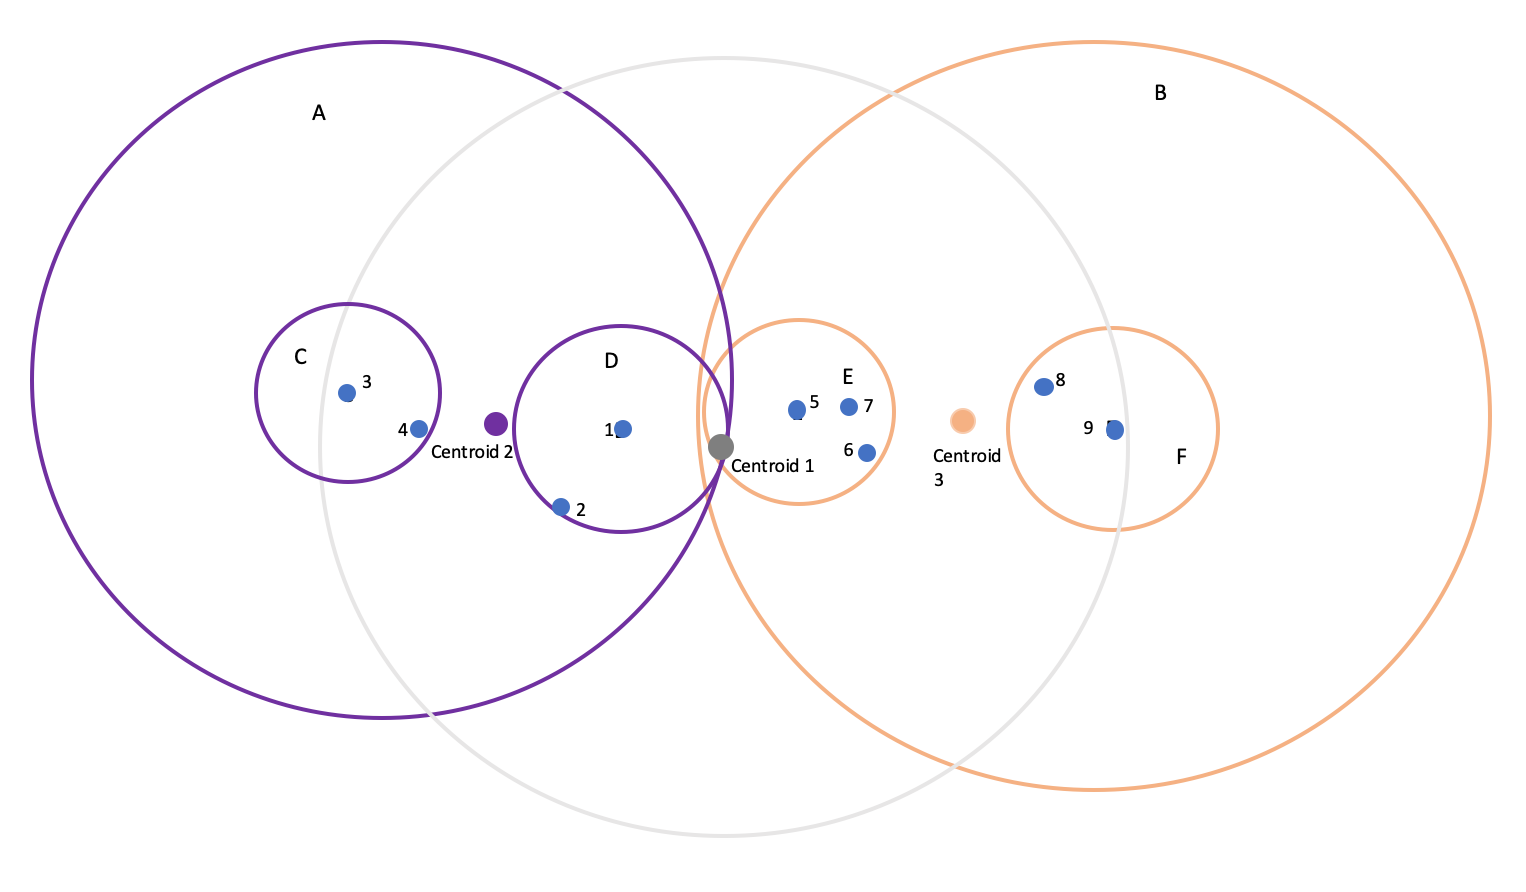
\includegraphics[width=300pt,height=180pt]{pictures/ball_tree.png}
    \caption{A demonstration of the Ball-tree algorithm with 9 datapoints having 2 dimensions x and y.\cite{kd_tree}}
    \label{fig:ball_tree}
\end{figure} 
Fast nearest neighbor searches are facilitated by this hierarchical arrangement, allowing for the rapid elimination of entire subtrees during the search process. Ball trees are particularly useful in scenarios with high-dimensional data, offering improved efficiency over exhaustive search methods in applications such as clustering, classification and nearest neighbor queries. The steps for ball-tree algorithm are:
\begin{enumerate}
    \item \textbf{Point Selection }: A random data point is chosen as the center of the hypersphere \cite{omohundro1989five}.
    \item \textbf{Radius Calculation}: The radius of the hypersphere is calculated using distance metrics such as Euclidean distance or Manhattan distance \cite{omohundro1989five}.
    \item \textbf{Datapoint Assignment}: Data points are assigned to the current node \cite{omohundro1989five}.
    \item \textbf{Recursive Process}: The process is repeated by selecting new centers and radii \cite{omohundro1989five}.
\end{enumerate}
Thus, the memory consumption for the ball-tree algorithm is way more in comparison to the \ac{KD}-tree algorithm. Furthermore, it fails to provide good results in low-dimensional data. It results to inefficient search time for low dimensional queries. This \ac{KD}-tree is suitable for low dimensional static use cases like image recognition and nearest neighbor search in low to medium dimensional dataset. Whereas, the ball tree algorithm is suitable for data clustering in high dimensional spaces and nearest neighbor search in high dimensional datasets.

\vspace{5mm}

\textbf{Brute Force Algorithm}
A brute force algorithm is a straightforward and exhaustive search strategy that systematically examines all possible options until it finds the solution to a problem. It’s a general approach used for problem-solving when the problem size allows for detailed investigation. In the brute force method, it is iterated through each data point and the density is calculated by considering the distances to other points. However, due to their high time complexity, brute force methods are inefficient for large-scale problems.

\subsection{Evaluation Metrices}
This section gives an overview of the evaluation metrices used to compare the results of the different clustering algorithms evaluated in this thesis. It also provides the details of the metric used to compare how similar the objects in the test dataset are to the representative members of the entire dataset. 
\subsubsection{Metric for Clustering Algorithms}
It is evident how even the evaluation metrics using just the intrinsic features of the dataset are still not efficient in the presence of noise, outliers or non-convex clusters. As pointed out by the authors of \cite{jain1988algorithms}, "without a strong effort in this direction, cluster analysis will remain a black art accessible only to those true believers who have experience and great courage". The fact that this statement holds even today, 35 years after he said it is even more astonishing. To tackle the problem of inefficient evaluation metrics for non-convex clusters or where the different clusters have a difference in size Moulavi \textit{et. al.} proposed the \ac{DBCV} Index \cite{moulavi2014density}.

\subsubsection*{Density Based Cluster Validition Index}
\label{sec:dbcv}
The authors have utilised the theory of Hartigan's model of density-contour trees \cite{hartigan1975clustering}. The least dense region within a cluster and the most dense region outside a cluster is calculated with it which is analogous to computing the within cluster and between cluster density connectedness. As per the definition of Density Contour Trees \cite{hartigan1975clustering} by Hartigan, density based clusters are regions of high density which are separated by low density regions. Having such model as a backdrop, it is expected that a good clustering algorithm which generate clusters such that the least dense region within a cluster is still more dense as compared to regions surrounding a cluster. Traditional intrinsic measure based evaluation metrics uses distance between the datapoints to compute cluster-variance and then incorporates it with the separation between the clusters to eventually compute the quality of the clustering algorithm. But this is not the target for \ac{DBCV}. So a metric is proposed which is defined by densities instead of distances. \ac{DBCV} wants to take into account both the density and the shape of the cluster. So at first, the authors defined the concept of "all-points-core-distance"($a_{pts}coredist$). It is the inverse of the density of each object with respect to all other objects inside its cluster as given in Eq. \ref{eq:aptscoredist}.
\begin{equation}
  \label{eq:aptscoredist}
  \mathit{a_{pts}coredist(\textbf{o})}= \mathit{\left\{\frac{\sum_{i=2}^{n_i}\left(\frac{1}{KNN(\textbf{o},i)}\right)^d}{n_i - 1}\right\}^{-\frac{1}{d}}}.
\end{equation}
Using the above-mentioned equation, a symmetric reachability distance is defined which is then utilized to generate the \ac{MST} inside each clusters. Because the \ac{MST}s are built on the transformed space of symmetric reachabilty distances, it is capable of capturing both the density and shape of the cluster. On using these \ac{MST}s, it is possible to find the least dense region within each of the clusters and the most dense regions between the pair of clusters. As per the definitions provided by the authors, $\textbf{O} = {o_1, o_2, ...., o_n}$ is the dataset containing $n$ objects in the $\mathbb{R}^d$ feature space. $\textbf{Dist}$ is an $n \times n$ matrix of pairwise distance $d(o_p,o_q)$ between the objects of the dataset, such that $o_p,o_q \in \textbf{O}$. $KNN(\textbf{o},i)$ is the distance between the object $o$ and its $i^{th}$ nearest neighbor. $C=({C_i},N) 1 \leq i \leq l$ is the results returned by the clustering algorithms having $l$ clusters and a set of $N$ noise objects. $n_i$ is the size of the $i^{th}$ cluster and $n_N$ is the number of objects in that particular cluster. To get an estimate of the density of an object within a cluster, traditional approaches use the notion of taking the inverse of the threshold distance required to find $K$ objects within this threshold \cite{hartigan1975clustering, campello2012simpler}. But a drawback of this method would be that it is required to decide the value of the parameter $K$, which is not desirable. 

\vspace{5mm}

Moreover, with this approach, the density of the object is dependent to its distance from only one other object i.e. the $k^th$ nearest neighbor. This approach is not as robust as compared to considering more objects in its neighborhood as done in Gaussian distribution kernel density estimation. Thus, in order to propose a more robust density estimation, the use of a new parameterless core distance is proposed which can be elucidated as the inverse of a density estimate and thus, can be used in defining the \ac{MRD}. So now instead of using just one point in the cluster, all the points are taken into account such that the objects closer to it contribute to the density more as compared to the objects further away. It can be seen in Eq. \ref{eq:aptscoredist}, that the inverse of the $KNN$ distances raised to the power of dimensions is calculated such that closer objects gets a higher weight as compared to further objects. This effect can further be increased by using squared Euclidean distance instead of Euclidean distances. Also, as per the definition of \ac{MRD}\cite{lelis2009semi}, the core distance of an object is compared to the distances of the object to other objects in the cluster. Hence, the core distance needs to be comparable to these distances. For each object $\textbf{o}$ in the cluster, the "all-points-core-distance" $a_{pts}coredist(\textbf{o})$ lies between the second and the last nearest neighbor distance of the object\cite{moulavi2014density} as in Eq. \ref{eq:knndist}. 

\begin{equation}
  \label{eq:knndist}
  \mathit{KNN(\textbf{o},2)} \leq \mathit{a_{pts}coredist(\textbf{o})} \leq \mathit{KNN(\textbf{o},n)}.
\end{equation}

Moreover, the core distance is approximated to the distance of the object to its $k^{th}$ nearest neighbor such that $k$ is not too large. This means, that only a small neighborhood of the object is to be considered. Furthermore, let n objects be uniformly distributed random variables in a d-dimensional unit hypersphere. Then the core distance of object $\textbf{o}$ is given by Eq. \ref{eq:aptsln}.\cite{moulavi2014density}

\begin{equation}
  \label{eq:aptsln}
  \mathit{a_{pts}coredist(\textbf{o})} = \mathit{\ln(n)^{-\frac{1}{d}}}.
\end{equation}

The core distance of the object $\textbf{o}$ is approximately equal to the same nearest neighbor distance and is independent of the dimension of the data space, if the objects are uniformly distributed. If the dataset doesn't have a uniform distribution, which is the case for most real world datasets, only the first property holds i.e. the density of the object doesn't depend on just one other object but on all objects in the cluster.\cite{moulavi2014density}

\vspace{5 mm}

Now the $a_{pts}coredist$ is used to compute the symmetric reachability distance which is delved into deeper in the following paragraphs. As per the authors, the \ac{MRD} between two objects $o_i$ and $o_j$ as in Eq. \ref{eq:mut_reach_dist}.

\begin{equation}
  \label{eq:mut_reach_dist}
  \mathit{d_{mreach}(\textbf{o}_i, \textbf{o}_j)} = \mathit{max\{a_{pts}coredist(\textbf{o}_i), a_{pts}coredist(\textbf{o}_j), d(\textbf{o}_i, \textbf{o}_j)\}},
\end{equation}

where $ d(\textbf{o}_i, \textbf{o}_j)$ is the Euclidean distance between object $\textbf{o}_i$ and $\textbf{o}_j$. Once the \ac{MRD} is computed, it could now be used to generate the mutual reachability graph where the objects are the different vertices and the graph and the \ac{MRD} calculated above are the edge weights between the pair of vertices. Now with the set of objects $\textbf{O}$ and the mutual reachability graph $G$, the \ac{MST} of graph $G$ is computed as $\ac{MST}_{\ac{MRD}}$. So a quick overview of the process of \ac{DBCV} would be that for a single cluster $C_i$ having objects $O$, the $a_{pts}coredist$ of each object in the cluster is calculated. This is then used to computer the \ac{MRD} between all pair of objects in the cluster. Depending on the \ac{MRD}, the \ac{MST} is generated. This process is then performed for all the clusters generated by the clustering algorithm, eventually giving rise to $l$ \ac{MST}s if the clustering algorithms returns $l$ clusters in total. Thus, it can noticed that the number of \ac{MST}s increase linearly with the increase in the number of clusters. Also, the size of the tree depends on the number of objects in the clusters and thus, can blow up exponentially in case of very large datasets having a lot of elements in each cluster.  

\vspace{5 mm}

From the \ac{MST}s generated above, a new measure to validate the quality of the clustering algorithm depending on the density sparseness and density separation is crafted as explained below. The \ac{DSC} $C_i$ can be visualized as the least dense region within the cluster and thus, can be obtained from the maximum edge weight of the $\ac{MST}_{\ac{MRD}}$ of that particular cluster. On the other hand, \ac{DSPC} $C_i$ and $C_j$ where $1 \leq i,j \leq l, i \neq j$  can be visualized as the region of highest density in between adjacent clusters and can be formulated as the minimum \ac{MRD} between the objects of a cluster to the objects of its neighboring cluster. The \ac{DSC} and the \ac{DSPC} together then give the validity index of a cluster as in Eq. \ref{eq:val_index}.
\begin{equation}
  \label{eq:val_index}
  \mathit{V_C(C_i)} = \mathit{\frac{\underset{1 \leq j \leq l, i \neq j}{min}\left(\ac{DSPC}(C_i,C_j)\right) - \ac{DSC}(C_i)}{max\left(\underset{1 \leq j \leq l, i \neq j}{min}\left(\ac{DSPC}(C_i,C_j)\right) - \ac{DSC}(C_i)\right)}}.
\end{equation}
Once the validity index of each cluster is calculated, the final \ac{DBCV} score of the clustering algorithm can be defined as the weighted average of the validity index of all the clusters in $C$ generated by the clustering algorithm as in Eq. \ref{eq:dbcv}. It is to be noted that even if noisy elements aren't explicitly present in the formula as a separate cluster but it does however implicitly affects the overall score as the weighted average takes into consideration both the cardinality of individual clusters as well as the total number of elements in the dataset, which includes noise and outliers. 
\begin{equation}
  \label{eq:dbcv}
  \mathit{\ac{DBCV}(C)} = \mathit{\sum_{i=1}^{l}\frac{|C_i|}{|O|}V_C(C_i)}.
\end{equation}
If a cluster has better density compactness within the cluster as compared to density separation in between adjacent clusters, than the validity index of the cluster would take a positive value. On the other hand, if the density outside the cluster separting it from adjacent clusters is more than density compactedness inside the cluster than it would take a negative value. Thus, the \ac{DBCV} score can vary in the range $[-1,1]$ where greater \ac{DBCV} score indicates to a better density-based clustering algorithm.

\subsubsection{Metric for Similarity in Point Clouds}
Hausdorff distance is commonly used to calculate the similarity between two point clouds. So if the set of representative members generalizes the entire dataset well enough, then each object in the test dataset would be very similar to atleast one object from the set of representative members. Hausdorff distance calculates how different one point cloud is to another. So, lower the Hausdorff distance, more similar are the point clouds to one another. Thus, for the a set of "good" representative members, the average distance from all objects in the test dataset to their corresponding nearest object in the representative set is minimum. Mathematically, Hausdorff distance is the measure of how far two subsets in a metric space. Intuitively speaking, the Hausdorff distance between two sets of points is lower when every point in one set is close to some point in the other set. In other words Hausdorff distance is the longest distance that needs to be covered when traveling from any point in one of the subsets to the closest point in the other subset. Let $(M,d)$ be a $d$-dimensional metric space and $X \subset M$, $Y \subset M$ are the two non-empty subsets of points, then the Hausdorff distance between $X$ and $Y$ is defined as in Eq. \ref{eq:hausdorff}.
\begin{equation}
    \label{eq:hausdorff}
    \mathit{d_H(X,Y)} := \mathit{\left\{max(\underset{x \in X}{sup} \; d(x,Y), \underset{y \in Y}{sup} \; d(X,y))\right\}},
  \end{equation}
where $sup$ is the supremum operator and $d(a,B) := \underset{b \in B}{inf} \; d(a,b)$ is the distance from a point $a \in X$ to the subset $B \subseteq X$, where $inf$ is the infimum operator. Thus, in the context of point clouds the Hausdorff distance is defined as in Eq. \ref{eq:hausdorff_point_cloud}. If $P_1 = \{x_i \in \mathbb{R}^3\}_{i=1}^n$ and $P_2 = \{x_j \in \mathbb{R}^3\}_{j=1}^m$, then the maximum distance between any pair of nearest neighbors between the two point clouds is defined as in eq. \ref{eq:hausdorff_point_cloud}.
\begin{equation}
    \label{eq:hausdorff_point_cloud}
    \mathit{hausdorff(P_1, P_2)} := \mathit{\frac{1}{2} \underset{x \in P_1}{max}\lvert x - NN(x,P_2) \rvert + \frac{1}{2} \underset{x' \in P_2}{max}\lvert x' - NN(x',P_1) \rvert},
  \end{equation}
\subsection{Important Aspects of the Studies}
\subsubsection{Focus and Restrictions}
\label{sec:restrictions}
The aim of this thesis is to find "good" representative members of the dataset which can be used as source library for transfer learning approaches to be used in bin picking applications. in order to do so, it is necessary to evaluate the performance of the clustering algorithms. But calculating the cluster evaluation metric like \ac{DBCV} for a very large high dimensional data can be extremely time consuming and inefficient. In order to circumvent this issue, the evaluation is carried on smaller subset of the dataset. But in order to ensure that the results can be interpolated to the entire dataset, subsets of varying sizes of the dataset have been evaluated on to confirm that the conclusions are consistent. The dimensions of the latent space representations play a very crucial role when encoding the features of the objects in a dataset in lower dimensional space. But in order to accurately evaluate the performance of the clustering algorithms, the number of dimensions has to be reduced further to be able to utilize the \ac{DBCV} metric for evaluation of the clustering results. Moreover, to facilitate larger but denser clusters \ac{t-SNE} dimensionality reduction is utilized. In the event of a rapid reduction of dimensions for example 1024 to 2, it is advised in \cite{tsne_sklearn} to perform multi-step dimensionality reduction instead of reducing it in a single step. This helps in better handling of the noise and outliers \cite{scikit-learn}. To assure that the theoretical advice is coherent with the practical results, evaluations are carried on in this area, the results of which are documented in Ch. \ref{sec:pointnet_dim} and \ref{sec:conclu_dim}. The data generation procedure currently used at \ac{IPA} requires 24 hours for completely generating a single object. It was decided to use 3 available servers for this purpose of data generation. A practical and feasible choice of roughly two months is made for this purpose. Two months nearly equals to 1400 hours. Thus, the underlying derivation shows how the maximum possible number of representative objects is determined.
\begin{equation}
    \label{eq:time_calc}
    \begin{split}
        Total \; time &= \frac{Number \; of \; clusters}{Number \; of \; servers} * Time \; for \; each \; object\\
        Number \; of \; clusters &= \frac{Total \; time \times Number \; of \; server}{Time \; for \; each \; object}
        \\
        &= \frac{1400 \times 3}{24} = 175
    \end{split}    
\end{equation}

\subsubsection{Hardware and Environment Setup}
\label{sec:hardware}
All the aspects of this thesis work has been carried on into a single setup, a powerful workstation computer, ML-Lab-2 at \ac{IPA}. It is an Ubuntu server. The \ac{CPU} are two ”Quad Core Intel Xeon Silver 4112 @ 2.60 GHz” with a total installed \ac{RAM} of 275 GB. The system has two \ac{GPU} which are "Tesla V100-PCIE-32GB" and "NVIDIA GeForce RTX 3090" with 32 \ac{GB} and 24 \ac{GB} memory respectively. Each of the individual model training is executed on a single GPU. 
\cleardoublepage


